\documentclass{article}

\usepackage{kotex}
\usepackage{graphicx}
\usepackage[affil-it]{authblk}
\usepackage{mathtools}
\usepackage{amssymb}
\usepackage{amsthm}
\usepackage{geometry}
\usepackage{fancyhdr}
\usepackage{braket}
\usepackage{cite}
\usepackage{cancel}
\usepackage{subcaption}
\usepackage{enumitem}
\usepackage{color}
\usepackage{booktabs}
\usepackage{chemformula}
\usepackage{physics}
\usepackage{hyperref}

\newcommand{\vp}{\varphi}
\newcommand{\ve}{\varepsilon}

\newtheorem{theorem}{Theorem}
\newtheorem{definition}[theorem]{Definition}
\newtheorem{example}[theorem]{Example}
\newtheorem{lemma}[theorem]{Lemma}
\newtheorem{axiom}[theorem]{Axiom}
\newtheorem{remark}[theorem]{Remark}
\newtheorem{problem}[theorem]{Problem}
\newtheorem{exercise}[theorem]{Exercise}

\counterwithin{equation}{section}
\counterwithin{theorem}{section}


\geometry{a4paper,left=2cm,right=2cm,top=2.4cm,bottom=2.4cm}

\linespread{1.3}

\title{\textsf{Free Energy and Chemical Thermodynamics}}
\author[1]{Written by Eun Taek Kang\thanks{email: etkang03@gmail.com}}
\affil[1]{Department of Physics, Sogang University, Seoul 04107, Korea}

\date{Summer 2025, Sogang University}

\begin{document}

\pagestyle{fancy}
    %... then configure it.
    \fancyhf{}
    % Set the header and footer for Even
    % pages but omit the zone (L, C or R)
    \fancyhead[R]{\textsf{Prof.\ Hyeonjun Baek}}
    \fancyhead[L]{\textsc{Thermal Physics}}
    \fancyfoot[C]{\thepage}
    \fancyfoot[L]{\textbf{Sogang University}}
    \fancyfoot[R]{\textit{Department of Physics}}

\maketitle

\begin{abstract}
    백현준 교수님께서 2025년 1학기에 진행하는 열역학 기말고사 대비를 위해 만든 Note입니다. 이 문서는 Daniel V. Schroeder 저 An Introduction to Thermal Physics의 Chapter 5. Free Energy and Chemical Thermodynamics를 다루고 있습니다.
\end{abstract}

\newpage

\section{Free energy as available work}

\textbf{Thermodynamics Potentials}

우리는 어떠한 계의 에너지를 $U$로 표현했다. 이제, 3가지의 새로운 열역학 퍼텐셜들을 정의할 것이다.
\begin{equation}
    \boxed{H \equiv U + PV} \quad \boxed{F \equiv U - TS} \quad \boxed{G \equiv U - TS + PV}
\end{equation}
$H$는 엔탈피(enthalpy), $F$는 헬름홀츠 자유에너지(Helmholtz free energy), $G$는 깁스 자유에너지(Gibbs free energy)라고 한다. 

\begin{figure}[h]
\centering
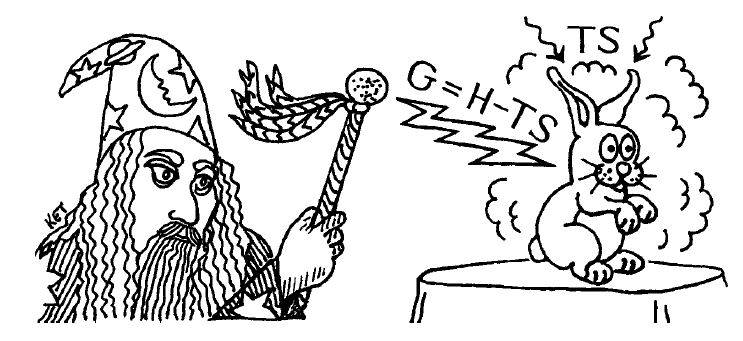
\includegraphics[width=0.6\linewidth]{images/fig1_1.png}
\end{figure}

토끼를 만드는 상상도에서 비유해보자. 탁자 위에 토끼를 만드는데 필요한 에너지는 엔탈피 $H=U+PV$이다. 그 중에 열 때문에 $TS$정도는 자연적으로 유입이 가능함. 따라서 마법사가 필요한건 깁스 자유에너지 $G=H-TS$만큼이 필요한거다. \underline{법사가 $G$만큼만 걸어줘도 토끼가 만들어져요!}

\begin{figure}[h]
\centering
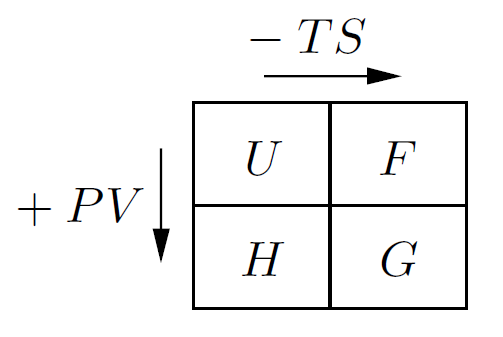
\includegraphics[width=0.4\linewidth]{images/fig1_2.png}
\end{figure}

\noindent
\textcolor{red}{따라서, 우리는 위의 diagram을 필히 외워두도록 하자. 헷갈릴 때 저 diagram을 이용하면 혼돈을 막을 수 있다.}

\begin{itemize}
    \item 온도 $T$가 일정할 때, $\Delta F = \Delta U - T\Delta S = Q + W - T\Delta S$이다. 
    
    $Q$는 가한 열, $W$는 계에 해준 일이다. 일반적으로 $Q \leq T\Delta S \ \Rightarrow \ \Delta F \leq W$이다. (엔트로피 안 생기면 등호 성립) 특히, $W$는 환경의 수축 및 팽창에 의한 일도 포함한다.

    \item 온도 $T$와 압력 $P$가 일정할 때, $\Delta G = \Delta U - T \Delta S + P \Delta V = Q + W - T \Delta S + P \Delta V$이다.
    
    이때, $W = -P\Delta V + W_{\text{other}}$이다. ($-P\Delta V$는 환경에 의한 일), 역시 $Q \leq T\Delta S$이므로, $\Delta G \leq W$이다!
\end{itemize}

특히나 깁스 자유에너지를 다음과 같이 계산하는 방법은 자주 쓰인다.
\begin{equation}
    \Delta G = \Delta H - T \Delta S
\end{equation}

\newpage

\noindent
\textbf{Electrolysis, Fuel cells, and Batteries} \textcolor{blue}{(Free energy example!)}

\vspace{1mm}
물의 전기 분해부터 살펴보자. $\ch{H2 O} \rightarrow  \ch{H2} + \dfrac{1}{2} \ch{O2}$인건 명백하다.

\begin{figure}[h]
\centering
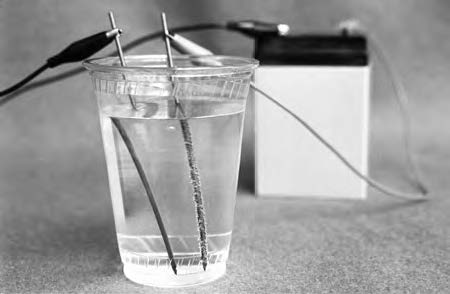
\includegraphics[width=0.35\linewidth]{images/fig1_3.jpeg}
\end{figure}

여기서, 깁스 자유 에너지는 다음과 같다.
\begin{equation}
    \Delta G = \Delta H - T \Delta S = \Delta U + P\Delta V - T \Delta S
\end{equation}
1몰의 물에서 일어나는 에너지 출입의 모식도는 이렇다.

\begin{figure}[h]
\centering
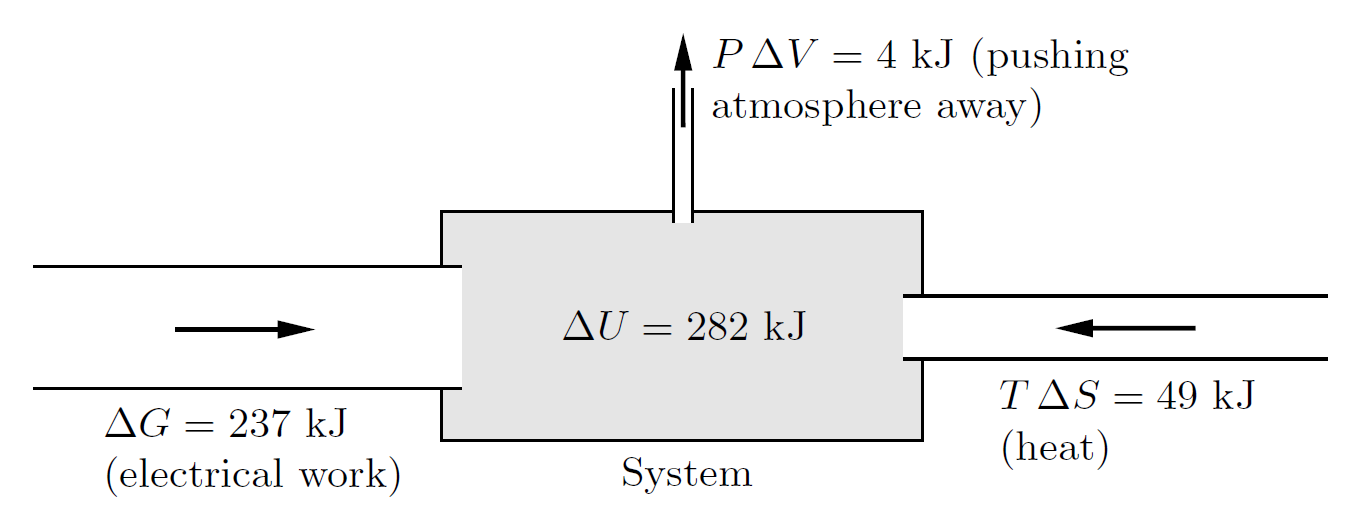
\includegraphics[width=0.65\linewidth]{images/fig1_4.png}
\end{figure}

계에 해준 일과 열에 의한 유입 에너지를 계산해보자.\footnote{131, 205, 70같은 숫자는 화학책 표에서 찾는다. 크게 신경쓸 값은 아님.}
\begin{equation}
    P \Delta V = (\Delta n) R T = (1 + 1/2) \cdot (8.31) \cdot (293) \approx 4 \text{kJ}
\end{equation}
\begin{equation}
    T \Delta S = \left[ \left( 131 + \frac{1}{2} \cdot 205 \right) -70 \right] \cdot (293) \approx 49 \text{kJ}   
\end{equation}
다음은 수소 연료를 알아보자. 

\begin{figure}[h]
\centering
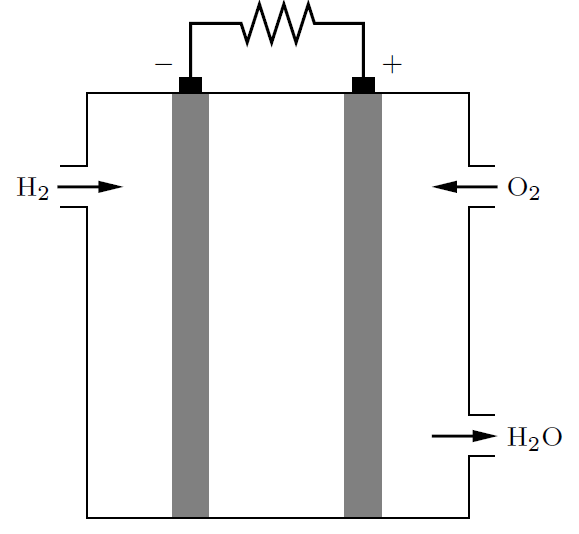
\includegraphics[width=0.3\linewidth]{images/fig1_5.png}
\end{figure}

이 과정에선 반응식이 반대로 $\ch{H2 O} \leftarrow  \ch{H2} + \dfrac{1}{2} \ch{O2}$이다. 또한, 위의 모식도의 모든 화살표 방향이 반대가 되고, $\Delta U = -282$ kJ가 된다. 또한, 이상적인 연료의 효율성을 계산하면 다음과 같다.
\begin{equation}
    \frac{|\Delta G|}{|\Delta U|} = \frac{237}{286} \approx 83 \%
\end{equation}

\newpage

마지막으로, 배터리를 알아볼 것이다. 배터리는 다음과 같은 모식도를 가진다.

\begin{figure}[h]
\centering
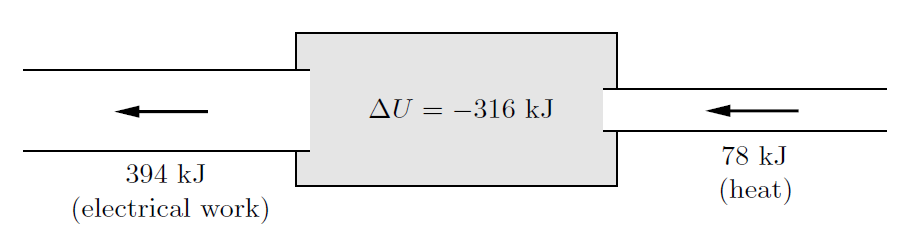
\includegraphics[width=0.6\linewidth]{images/fig1_6.png}
\end{figure}

\noindent
신기한 점은, 배터리는 $\Delta U \approx \Delta H$이고, $\Delta F \approx \Delta G$이다. 배터리의 반응식은 다음과 같다.
\begin{equation*}
    \ch{Pb} + \ch{Pb O2} + \ch{4 H+} + \ch{2 SO4 ^{2-}} \rightarrow \ch{2 Pb SO4} + \ch{2 H2 O}
\end{equation*}
이는 다음의 3단계로 반응이 일어난다.
\begin{align*}
    \text{in solution} &: \ch{2 SO4 ^{2-}} + \ch{2 H+} \rightarrow \ch{2 HSO4-}\\
    \text{at $-$ electrode} &: \ch{Pb}  + \ch{HSO4-} \rightarrow \ch{PbSO4} + \ch{H+} + \ch{2 e-}\\
    \text{at $+$ electrode} &: \ch{PbO2} + \ch{HSO4- } + \ch{3 H+}  + \ch{2 e-} \rightarrow \ch{Pb SO4} + \ch{2 H2O}
\end{align*}
또한, 이때 전자 1개 당 해준 전기적 일은 다음과 같다.
\begin{equation}
    \frac{394 \text{kJ}}{2 \cdot 6.02 \times 10^{23}} = 3.27 \times 10^{-19} \text{J} = 2.04 \text{eV}
\end{equation}

\noindent
\textbf{Thermodynamic identities}

앞서, 우린 아주 중요한 에너지의 전미분을 배웠다.
\begin{equation}
    \boxed{dU = Tds - PdV + \mu dN}
\end{equation}
헬름홀츠 자유에너지 $F = U - TS$에 적용해보자.
\begin{equation}
    dF = dU - Tds - SdT = (Tds - PdV + \mu dN) - Tds - SdT = \boxed{-PdV + \mu dN - SdT}
\end{equation}
따라서, 우리는 헬름홀츠 자유에너지는 $T, V, N$에 대한 함수 $F(T,V,N)$으로 쓸 수 있고, 다음 identities가 성립한다.
\begin{equation}
    \boxed{P = -\left( \frac{\partial E}{\partial V} \right)_{T, N}} \quad \boxed{\mu = \left( \frac{\partial E}{\partial N} \right)_{T, V}} \quad \boxed{S = -\left( \frac{\partial E}{\partial T} \right)_{V, N}}
\end{equation}
이제, 다음 3가지 중요한 전미분을 기억하자.
\begin{align}
    \boxed{dS = \frac{1}{T} dU + \frac{P}{T} dV - \frac{\mu}{T} dN} \quad \boxed{dU = T\,dS - P\,dV + \mu\,dN} \quad \boxed{dF = -S\,dT - P\,dV + \mu\,dN}
\end{align}
이로부터, 중요한 편미분 identity들을 얻을 수 있다. 진짜 개중요하니 알아두자. 모르면 쉽지 않다.

\begin{table}[h]
\centering
\begin{tabular}{@{}cccc@{}}
\toprule
 & $S(U,V,N)$ & $U(S,V,N)$ & $F(T,V,N)$ \\ \midrule
$T$ &
  $\dfrac{1}{T} = \left( \dfrac{\partial S}{\partial U} \right)_{V, N}$ &
  $T = \left( \dfrac{\partial U}{\partial S} \right)_{V, N}$ &
  $T \text{ is given.}$ \\
$P$ &
  $\dfrac{P}{T} = \left( \dfrac{\partial S}{\partial V} \right)_{U, N}$ &
  $P = - \left( \dfrac{\partial U}{\partial V} \right)_{S, N}$ &
  $P = - \left( \dfrac{\partial F}{\partial V} \right)_{T, N}$ \\
$\mu$ &
  $- \dfrac{\mu}{T} = \left( \dfrac{\partial S}{\partial N} \right)_{U, V}$ &
  $\mu = \left( \dfrac{\partial U}{\partial N} \right)_{S, V}$ &
  $\mu = \left( \dfrac{\partial F}{\partial N} \right)_{T, V}$ \\ \bottomrule
\end{tabular}
\caption{Thermodynamic Potentials의 identities}
\label{tab:1}
\end{table}

\newpage

깁스 자유 에너지에 대한 identities도 뽑을 수 있는데, 먼저 깁스 자유 에너지의 전미분을 구해보자.
\begin{align}
    \boxed{G = U - TS + PV } \quad \rightarrow \quad dG &= dU - TdS- SdT + PdV + VdP\\ \nonumber
    &= (\cancel{TdS} - \cancel{PdV} + \mu dN) - \cancel{TdS} - SdT + \cancel{PdV} + VdP\\
    &\Rightarrow \boxed{ dG = -SdT + VdP + \mu dN}
\end{align}
따라서, $G$를 변수들을 통해 나타내주면 $G = G(S,P,N)$이고, 편미분 identities는 다음과 같다.
\begin{equation} \label{eq:1-14}
    \boxed{S = - \left( \frac{\partial G}{\partial T} \right)_{P,N}} \quad \boxed{V = \left( \frac{\partial G}{\partial P} \right)_{T,N}} \quad \boxed{\mu = \left( \frac{\partial G}{\partial N} \right)_{T,P}}
\end{equation}
이것들은 전부 \underline{system이 단일 종류의 입자라는 가정}에서나 맞고, 만약 다종류 입자 system이라면 화학 퍼텐셜 $\mu$들이 달라진다. $\mu d N$이 그들의 전체 합으로 대체되어야 한다. 따라서, 예를 들어 입자가 $k$개면 다음과 같다.
\begin{equation}
    \mu_1 = \left( \frac{\partial G}{\partial N_1} \right)_{T, P, N_2, N_3, \cdots, N_k} \quad \mu_2 = \left( \frac{\partial G}{\partial N_1} \right)_{T, P, N_1, N_3, \cdots, N_k}
\end{equation}

\section{Free Energy as a force toward equilibrium}

고립계에선 보통 엔트로피는 증가한다. 근데, 비고립계에선 어떨까??

\begin{figure}[h]
\centering
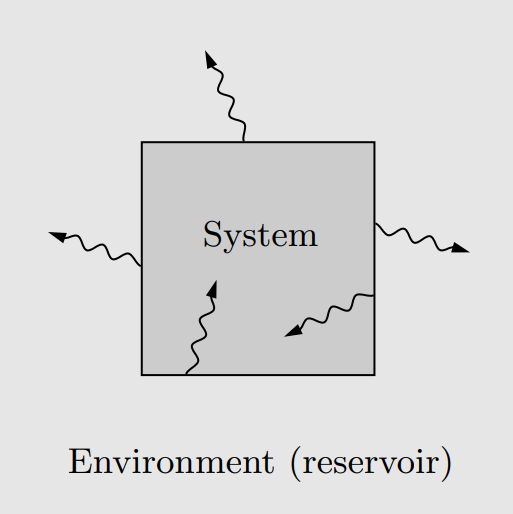
\includegraphics[width=0.25\linewidth]{images/fig2_1.png}
\end{figure}

이렇게 주변이랑 에너지 교환은 가능한 고립계를 생각해보자.\footnote{외부 환경이랑 에너지 교환마저 안되면 이걸 닫힌계(closed system)라고 한다.} 엔트로피는 크게 표현해주면 다음과 같다.
\begin{equation}
    dS_{\text{total}} = dS_s + dS_R 
\end{equation}
이때, \textcolor{blue}{$T,V,N$은 고정된 상태이다.} 그러면 다음 식에 의하여 \underline{에너지 $U$만 변할 수 있다.}
\begin{equation}
    dS = \frac{1}{T}dU + \frac{P}{T}dV - \frac{\mu}{T} dN
\end{equation}
엔트로피는 에너지에 의존하는 변수이므로, $S(U)$ 형태로 분석해보자.
\begin{align}
    S_{\text{tot}} &= S_s(U_s) + S_R (U_{\text{tot}} - U_s)\\ \nonumber
    &\approx S_s(U_s) + S_R (U_{\text{tot}}) - U_s \left( \frac{\partial S_R}{\partial U_R} \right)_{V,N} \quad (U_s \ll U_\text{tot}, \ \text{Taylor Expansion})\\
    &= S_R (U_{\text{tot}}) - \frac{1}{T_s} \cdot U_s + S_s (U_s) \qquad \qquad  \left[ \left( \frac{\partial S_R}{\partial U_R} \right)_{V,N} = \frac{1}{T_R} = \frac{1}{T_S} \right]
\end{align}
따라서 $V,N,T$가 일정할 때, $S$가 증가할 수록, $F$는 감소한다. 여기서 $\Delta F \leq W$에 의하면, 따로 계에 일을 가하지 않으면 $F$는 감소한다.

\newpage

만약, $T,P,N$이 고정되어 있다면 어떨까? 쉽게 말해 계의 부피도 변할 수 있단 가정을 해보자는 것이다. 수식적으론, $S$를 결정하는데 $U, V$가 관여한다는 것이다.\footnote{교과서엔 자세하게 없는 내용이다.}
\begin{align}
    S_{\text{tot}} &= S_s(U_s , V_s) + S_R (U_{\text{tot}} - U_s , V_{\text{tot}} - V_s)\\ \nonumber
    &\approx S_R(U_{\text{tot}}, V_{\text{tot}}) - \left( \frac{\partial S_R}{\partial U_R} \right)_{V,N} U_s - \left( \frac{\partial S_R}{\partial V_R} \right)_{U,N} V_s + S_s(U_s, V_s)\\
    &= S_R(U_{\text{tot}}, V_{\text{tot}}) - \frac{U_s}{T_s} - \frac{P_s}{T_s} \cdot V_s + S_s(V_s, U_s) \quad \left[ \left( \frac{\partial S_R}{\partial V_R} \right)_{U,N} = \frac{P_R}{T_R} = \frac{P_S}{T_S} \right]
\end{align}
따라서, $T,P,N$이 일정할 때, $S$가 증가할 수록 $G$는 감소한다. 이 역시 $\Delta F \leq W$에 의한 결과이다. 그러고 나서 $F$와 $G$의 정의를 다시 보자.
\begin{equation}
    F \equiv U - TS \qquad G \equiv U - TS + PV
\end{equation}
이를 종합하면, \textbf{고온에선 $S$가, 저온에선 $U$가} 에너지의 경향성을 지배한다고 할 수 있다.

\vspace{3mm}\noindent
\textbf{Minimum of $F=U-TS$}

\begin{center}
    \fbox{헬름홀츠 자유에너지($F$)는 equilibrium(평형점)에서 최소이다.}    
\end{center}
이 명제에 의하여 직관적으로 다음을 얻을 수 있다.
\begin{equation}
    \mu = \left( \frac{\partial F}{\partial N} \right)_{T,V}, \qquad P = - \left( \frac{\partial F}{\partial V} \right)_{T,N}
\end{equation}
다음과 같이 두 system이 마주보고 겹쳐 있다 하자.

\begin{figure}[h]
    \centering
    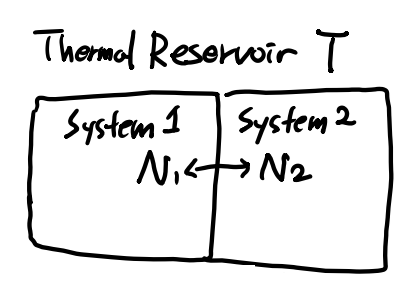
\includegraphics[width=0.3\linewidth]{images/fig2_2.png}
\end{figure}

\noindent
처음으로, $V_1, V_2$는 고정이고, $N_1 + N_2 = N_{\text{tot}}$라고 하자. 평형점에선 헬름홀츠 자유에너지의 합 $F_1 + F_2$는 최소다. 따라서
\begin{equation}
    \frac{\partial (F_1 + F_2)}{\partial N_1} = 0 = \frac{\partial F_1}{\partial N_1} + \frac{\partial F_2}{\partial N_2} = \frac{\partial F}{\partial N_1} - \frac{\partial F_2}{\partial N_2} \quad \Rightarrow \quad \frac{\partial F_1}{\partial N_1} = \frac{\partial F_2}{\partial N_2} \ \ (\mu_1 = \mu_2)
\end{equation}
만약, $N_1, N_2$가 고정되어 있고, $V_1 + V_2 = V$라고 한다면, 다음이 성립한다.
\begin{equation}
    \frac{\partial F_1}{\partial V_1} = \frac{\partial F_2}{\partial V_2} \ \ (P_1 = P_2)
\end{equation}

\newpage

\noindent
\textbf{Extensive and Intensive quantities}

\begin{figure}[h]
    \centering
    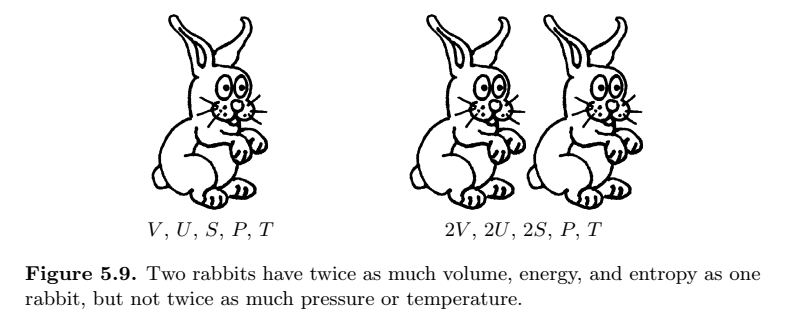
\includegraphics[width=0.7\linewidth]{images/fig2_3.png}
\end{figure}

열역학에서 변수들이 상당히 많이 나왔다. 이들은 다음과 같다.
\begin{equation*}
    U, \ V, \ N, \ S, \ T, \ P, \ \mu, \ H, \ F, \ G, \ m, \ \rho, \ C, \ c
\end{equation*}
\cancel{진짜 드럽게도 많다..} 여하튼, 이것들을 크게 2가지 종류의 변수로 구분할 수 있다. \textbf{크기변수}(extensive)는 계를 2배로 하면 함께 2배가 되는 물리량이고, \textbf{세기변수}(Intensive)는 함께 2배가 되지 않는 물리량이다. 위의 토끼 그림을 보면 된다. 따라서 분류하면 다음과 같다.
\begin{align*}
    \text{Extensive: }&V, \ N, \ S, \ U, \ H, \ F, \ G, \ m,\ C \\
    \text{Intensive: }&T, \ P, \ \mu, \ \rho, \ c
\end{align*}
Thermodynamic Identity나 Free Energy를 보면 다음과 같다.
\begin{align}
    dU &= TdS - PdV + \mu dN &(U, S, V, N \text{ Ex. } / \ T, P, \mu \text{ In.})\\
    F &= U - TS &(U, S \text{ Ex. } / \ T \text{ In.})\\
    G &= U + PV - TS &(U, S, V \text{ Ex. } / \ T, P \text{ In.})
\end{align}

\noindent
\textbf{Gibbs free energy and Chemical Potential}

깁스 자유 에너지의 전미분과 그로부터 얻는 관계는 다음과 같다.
\begin{align}
    dG = - SdT + VdP + \mu dN  \quad &\Rightarrow \quad G=G(T,P,N) = N \cdot Q(T,P)\\ \nonumber
    &\Rightarrow \quad \left( \frac{\partial G}{\partial N} \right)_{T,P} = Q(T,P) \ \ \text{by }(\ref{eq:1-14})\\
    &\Rightarrow \quad \mu = Q (T,P) \ \ \Rightarrow \ \ G = \mu N \label{eq:2-15}
\end{align}
이 식은 계에 입자를 1개 추가할 때마다 깁스 자유에너지가 $\mu$씩 증가함을 나타낸다. 이제, 다양한 종류의 입자들을 포함하면 (\ref{eq:2-15})를 다음과 같이 일반화할 수 있다.
\begin{equation}
    G = N_1 \mu_1 + N_2 \mu_2 + \cdots = \sum_i N_i \mu_i
\end{equation}
이제, $T,N$이 고정된 상태에서 (\ref{eq:2-15})를 결합시키면, 다음이 성립한다.
\begin{equation}
    \left( \frac{\partial \mu}{\partial P} \right)_{T,N} = \frac{\partial }{\partial P} \left( \frac{G}{N} \right)_{T,N} = \frac{1}{N} \left( \frac{\partial G}{\partial P} \right)_{T,N} = \frac{1}{N} \cdot V = \frac{kT}{P} \quad \text{(In ideal gas)}
\end{equation}
이제 양쪽을 $P^\circ$부터 $P$까지 적분해주면 다음과 같다. ($P^\circ$는 보통 1 atm으로 둔다.)
\begin{equation}
    \mu(T,P) = \mu(T, P^\circ) + kT \ln \left( \frac{P}{P^\circ} \right)
\end{equation}
이 식은, 압력이나 밀도가 변할 때, $\mu$는 어떻게 변하는지 보여준다.

\newpage

\section{Phase Transformations od Pure Substances}

상변화(phase transformation)란, 물질의 환경이 아주 미세하게 변화함에도 불구하고 그 성질이 불연속적으로 바뀌는 현상을 말한다. 우리는 이걸 깁스 자유에너지를 통해 이해해볼 것이다.

\begin{figure}[h]
    \centering
    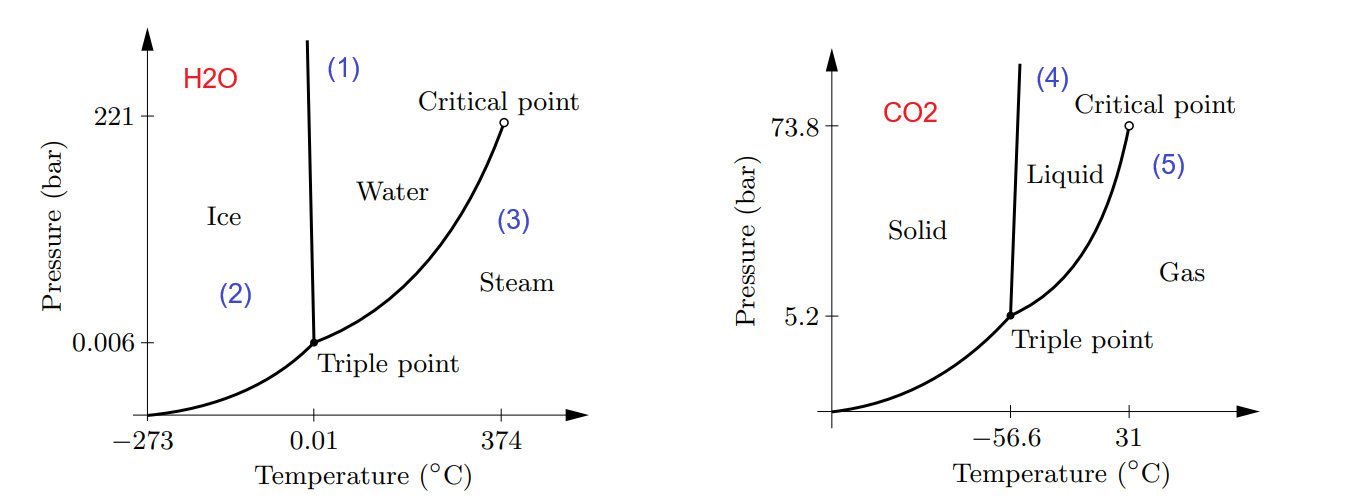
\includegraphics[width=0.95\linewidth]{images/fig3_1.png}
\end{figure}

\begin{enumerate}
    \item[(1)] 선 위에서는 두 개의 서로 다른 상이 공존할 수 있다.
    \item[(2)] 얼음은 특이하게도 압력을 높이면 녹는점이 낮아진다. 이는 얼음이 물보다 밀도가 작아서 그렇다. (곧 확인)
    \item[(3)] 액체-기체 경계선은 항상 양의 기울기를 가진다. 
    \item[(4)] 대부분의 물질은 압력이 증가하면 녹는점도 증가한다.
    \item[(5)] 유체에선 액체가 기체로 변할 때 불연속적인 변화가 없다.
\end{enumerate}

\noindent
\textbf{Helium's exotic phase transformation among all elements}

헬륨은 상 행동이 아주 특이하게 일어난다. 상변화 그림을 보자.

\begin{figure}[h]
    \centering
    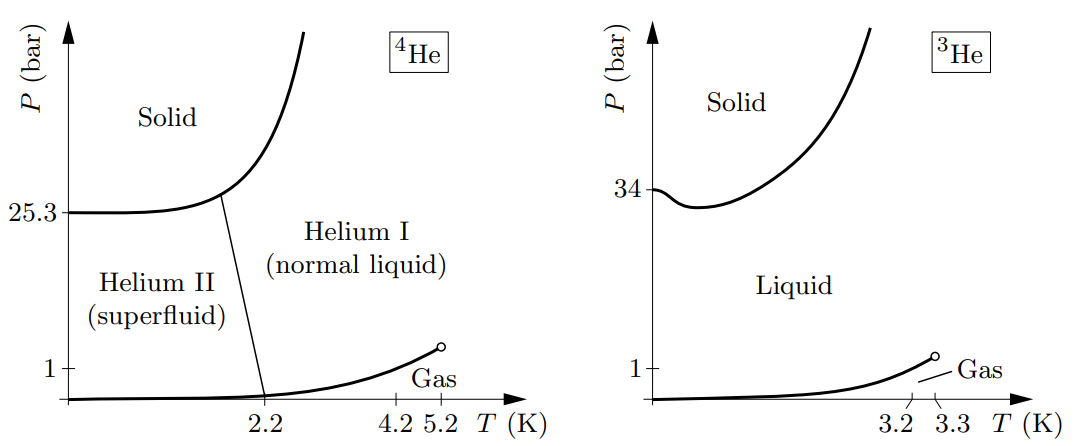
\includegraphics[width=0.78\linewidth]{images/fig3_2.png}
\end{figure}

\begin{itemize}
    \item 헬륨은 유일하게 0K(절대온도)에서도 액체 상태로 존재하는 원소이다.
    \item 특히, 헬륨 II같이 초유체 상태는 매우 특별한 성질들을 가지며, 그 중에는 무점성(zero viscosity)과 매우 높은 열전도율이 있다. (실험에서 액화 헬륨을 자주 쓰는 이유, 다만 아주 비싸다.)
\end{itemize}

\newpage

상변화를 일으키는데는 온도, 압력뿐 아니라 조성, 자기장 세기들도 영향을 미친다. 

\begin{figure}[h]
    \centering
    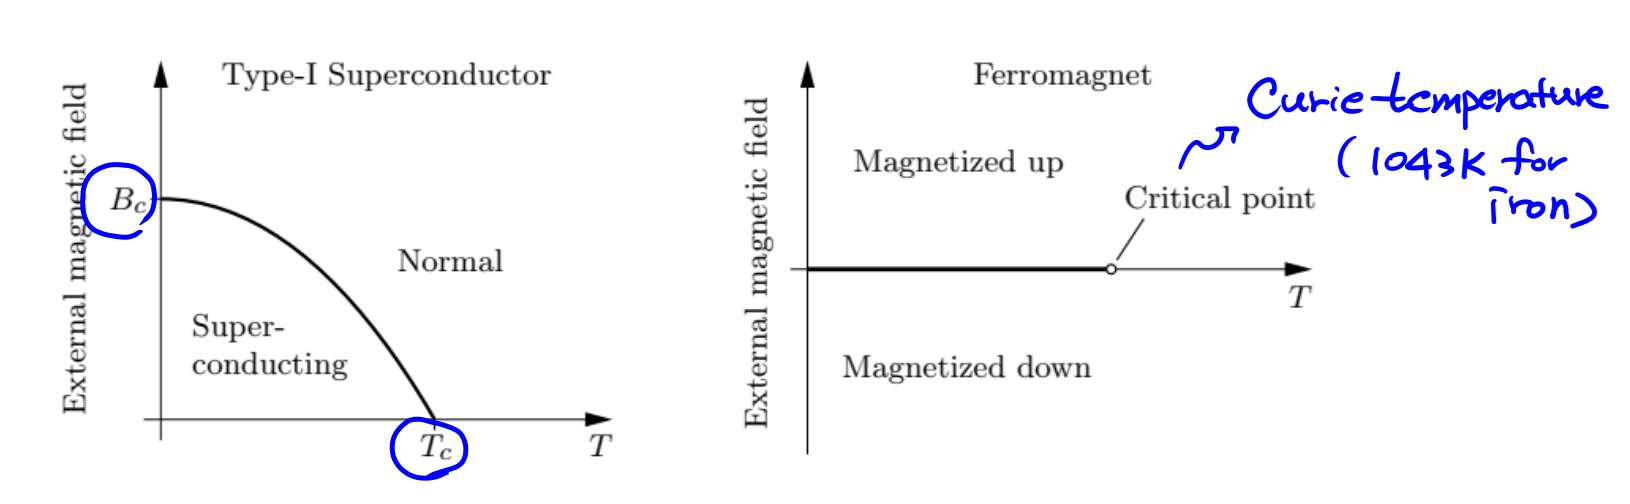
\includegraphics[width=0.9\linewidth]{images/fig3_3.png}
\end{figure}

\noindent
\textbf{Diamonds and Graphite}

(\ref{eq:1-14})에서 봤던 $V$에 대한 identity를 떠올리자.

\begin{figure}[h]
    \centering
    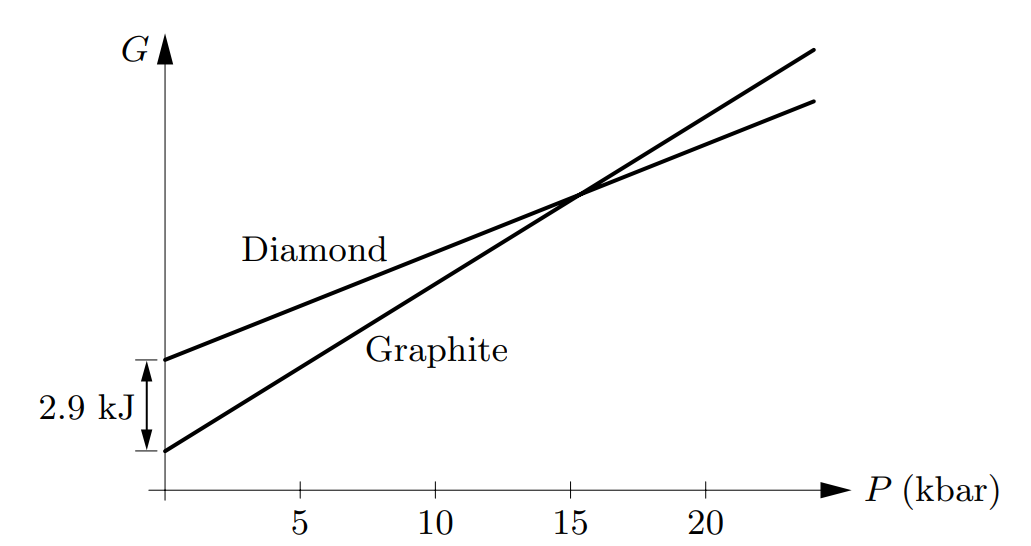
\includegraphics[width=0.6\linewidth]{images/fig3_4.png}
\end{figure}

\begin{itemize}
    \item 보통 상온, 상압에선 깁스 자유 에너지가 흑연이 다이아몬드보다 낮다. ($G_{\text{dia}} > G_{\text{gra}}$)
    \item 상압에선 흑연이 다이아몬드보다 안정된 상이다. 고로, 다이아몬드는 흑연으로 변하려 하지만, 상온에선 매우 느리게 일어난다.
    \item $V_{\text{gra}} > V_\text{dia}$에서, 그림의 $G-P$ 그래프 기울기는 흑연이 더 크다.
    \item 다만, 15 kbar 이상에선 흑연이 다이아몬드로 변한다.
\end{itemize}

\newpage

\noindent
\textbf{The Clausius-Calpeyron relation}

일단 다음과 같은 관계식을 기억해보자.
\begin{equation}
    \left( \frac{\partial G}{\partial T} \right)_{P,N} = -S, \quad \left( \frac{\partial S}{\partial P} \right)_{T,N} = V
\end{equation}
$P-T$ 그래프 그릴 때, 경계선의 기울기 양상은 두 상의 $S,V$ 차이와 연관이 있다. 

\begin{figure}[h]
    \centering
    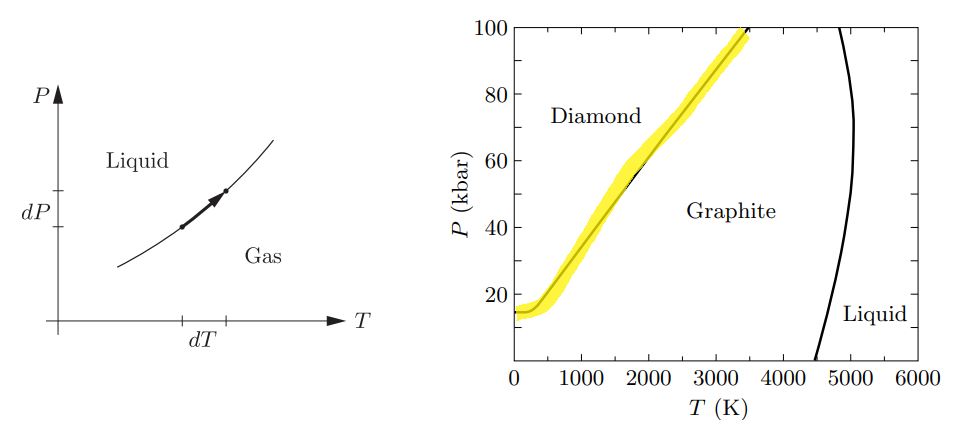
\includegraphics[width=0.8\linewidth]{images/fig3_5.png}
\end{figure}

기본적으로 상의 경계선에선, 두 상태의 깁스 자유 에너지가 같아야한다. ($dG_l = dG_g$) 다음 열역학적 identity를 다시 떠올리자.
\begin{equation}
    dG = -SdT + VdP
\end{equation} 
따라서, 다음이 성립한다.
\begin{equation}
    -S_{l} dT + V_l dP = -S_g dT  + V_g dP \ \ \Rightarrow \ \ \boxed{\frac{dP}{dT} = \frac{S_g - S_l}{V_g - V_l} = \frac{L}{\Delta V T}}
\end{equation}
여기서 $L$은 잠열이다. 우리는 박스 친 관계를 Clausius-Calpeyron relation이라고 한다. 실제로, 상온에서 1몰의 다이아몬드가 흑연이 될 때, 부피는 $1.9 \times 10^{-6}$m$^{3}$ 증가하고, 엔트로피는 3.4J/K 증가한다. 따라서,  상 경계의 기울기는 다음과 같다.
\begin{equation}
    \frac{dP}{dT} = \frac{\Delta S}{\Delta V} = \frac{3.4 \text{J/K}}{1.9 \times 10^{-6}\text{m}^3} = 18 \text{ bar/K}
\end{equation}

\noindent
\textbf{The Vander Waals model}

반데르 발스 방정식은 다음과 같다.
\begin{equation}\label{eq:3-5}
   \boxed{\left( P + \frac{aN^2}{V^2} \right)(V-Nb) = NkT}
\end{equation}
여기서, $a$는 분자의 양에 따른 비례상수, $b$는 분자가 이웃 분자와 닿아 있을 때, 분자 하나가 차지하는 최소한의 부피이다. 이 두 상수는 분자에 따라 다르다.

\begin{figure}[h]
    \centering
    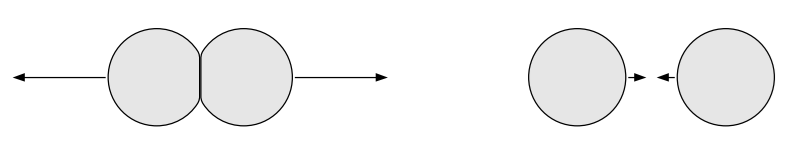
\includegraphics[width=0.7\linewidth]{images/fig3_6.png}
    \caption{두 분자가 너무 가까우면 밀어내고, 멀면 잡아 당긴다.}
\end{figure}

\newpage

Attraction potential energy는 $-aN^2/V$이고, 끌어당김에 의한 압력은 다음과 같다.
\begin{equation}
    P_{\text{att}} = - \left( \frac{\partial U}{\partial V} \right)_S = -\frac{d}{dV} \left(- \frac{aN^2}{V} \right) = - \frac{aN^2}{V^2}
\end{equation}
(\ref{eq:3-5})의 반데르발스 방정식을 그래프로 나타내면 다음과 같다. 그래프는 온도에 따라 달라진다.

\begin{figure}[h]
    \centering
    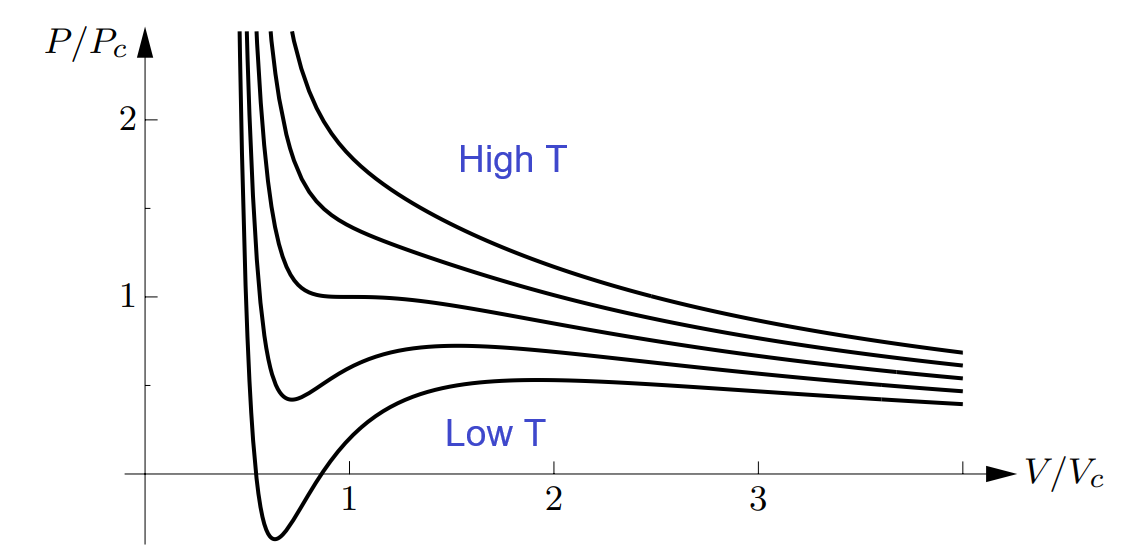
\includegraphics[width=0.55\linewidth]{images/fig3_7.png}
\end{figure}
$G$에 대한 열역학 항등식을 다시 떠올리자. ($dG = -SdT + VdP + \mu dN$) 만약 $N, V$가 고정이라면
\begin{equation}
    dG = VdP \quad \Rightarrow \quad \left( \frac{\partial G}{\partial V} \right)_{N,T} = V \left( \frac{\partial P}{\partial V} \right)_{N,T}
\end{equation}
반데르발스 방정식을 통해 나타낸 우변은 다음과 같다.
\begin{equation}
    \left( \frac{\partial P}{\partial V} \right)_{N,T} = -\frac{NkT}{(V-Nb)^2} + \frac{2aN^2}{V^3}
\end{equation}
이 결과를 통해 해석한 좌변은 이렇다.
\begin{align}
    \left( \frac{\partial G}{\partial V} \right)_{N,T} &= -\frac{NkTV}{(V-Nb)^2} + \frac{2aN^2}{V^2}\\
    &= -\frac{NkT(V-Nb)}{(V-Nb)^2} - \frac{NkT\cdot(Nb)}{(V-Nb)^2} + \frac{2aN^2}{V^2}\\
    &\Rightarrow  G = -NkT \ln (V-Nb) + \frac{NkT\cdot(Nb)}{(V-Nb)} - \frac{2aN^2}{V} + c(T,N)
\end{align}
여기서 $c(T,N)$은 양 변을 $V$에 대해 적분했기에 나오는 적분 상수이다.

\begin{figure}[h]
    \centering
    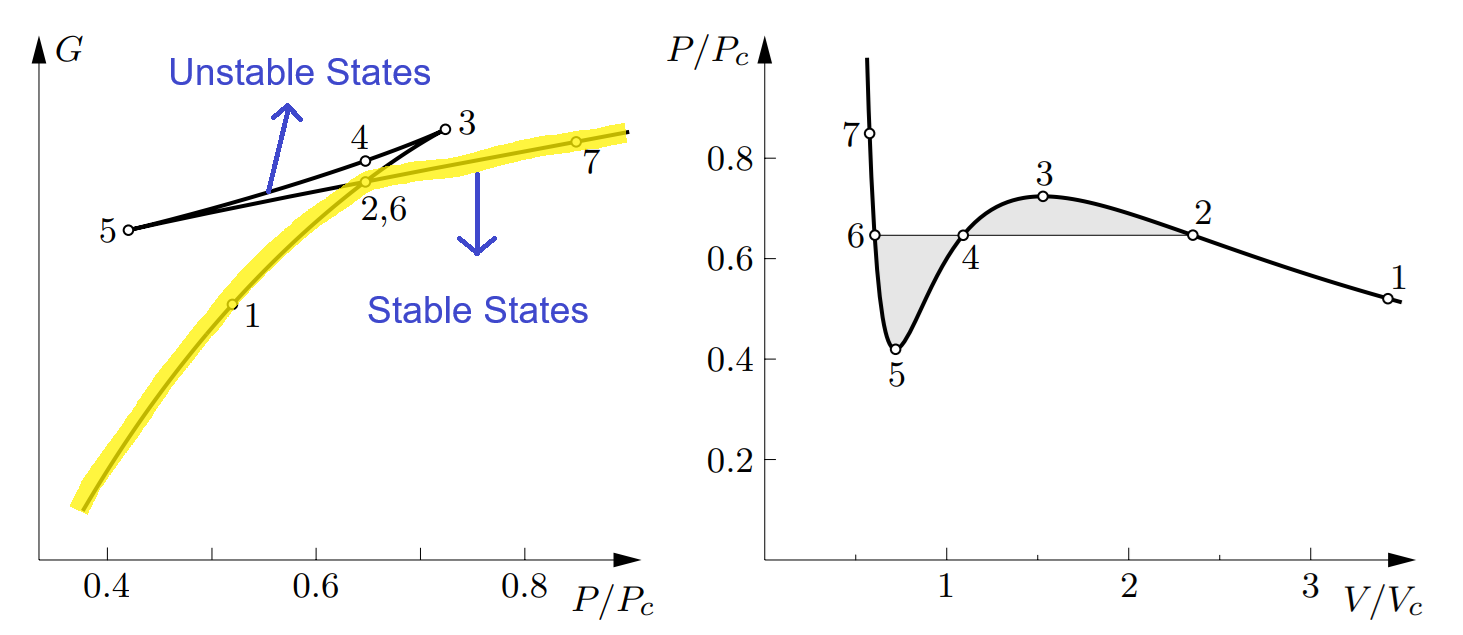
\includegraphics[width=0.75\linewidth]{images/fig3_8.png}
\end{figure}

$P-V$ 그래프에서 상변화 구간을 살펴보면, 압력이 점차 증가하면, 시스템은 점 2에서 점 6으로 곧바로 이동하며 부피가 갑자기 감소하게 된다. 다시 말해, 기체가 액체로 바뀌는 과정에서 압력은 일정하거나 천천히 증가하지만 부피는 급격히 줄어드는 현상을 나타낸다. 이처럼 \textcolor{blue}{반데르 발스 방정식 + 깁스 자유 에너지}를 이용하면 상변화를 아주 qualitatively하게 설명할 수 있다! 

\newpage

상변화가 일어나는 압력은 깁스 자유 에너지($G$) 그래프로부터 쉽게 구할 수 있다. 그러나, $PV$ diagram을 통해 바로 구할 수도 있는데, 다음과 같은 diagram을 보도록 하자. 앞서 본 그림을 회전시킨거다. 

\begin{figure}[h]
    \centering
    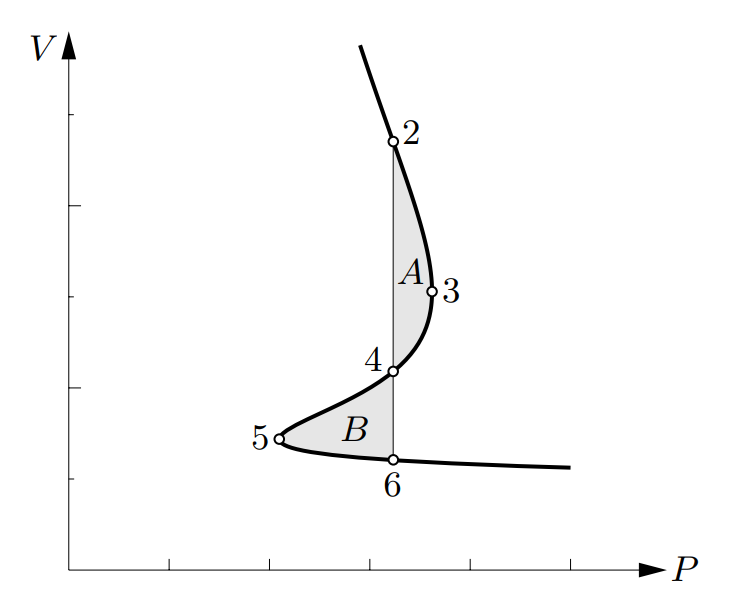
\includegraphics[width=0.4\linewidth]{images/fig3_9.png}
\end{figure}

\noindent
점 2에서 6까지 오름차순으로 삼각형 경로를 한 바퀴 돌면, \underline{깁스 자유 에너지의 전체 변화는 0}이다.
\begin{equation}
    0 = \oint_{\text{loop}} dG = \oint_{\text{loop}} \left( \frac{\partial G}{\partial P} \right)_T dP = \oint_{\text{loop}} V \, dP
\end{equation}
이는 곧 A와 B의 넓이차가 0임을 의미하기도 한다. 따라서, 상변화 압력은 $PV$ 곡선에서 enclosed area가 서로 같도록 하는 압력으로 결정되어야 성립한다.

\vspace{4mm}\noindent
\textbf{Maxwell Construction}

\begin{figure}[h]
    \centering
    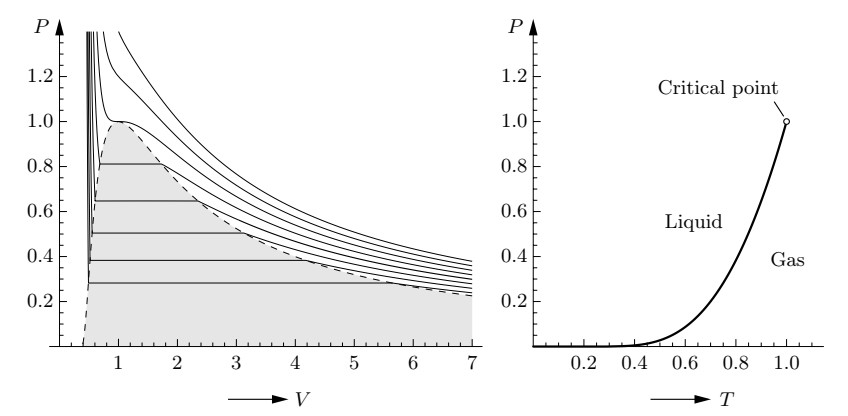
\includegraphics[width=0.75\linewidth]{images/fig3_10.png}
\end{figure}

\newpage

\section{Phase Transformation of Mixture}

아주 예전에 우리가 끓는점 배웠던걸 생각해보자. 물이랑 에탄올을 섞으면 78$^\circ$C에서 에탄올 한 번 날아가고, 100$^\circ$C에서 한 번 날아갔다. 그러나 혼합물은 그렇게 무 자르듯 두 온도에서 상변화가 일어나지 않았다. 따라서 순수 성분의 끓는점만 보고 혼합기체의 상전이를 예측하는 것은 부정확함. 그런고로, \underline{혼합물의 상평형 곡선}을 통해 해석하는 것이 바람직하다. 이번 절에선 혼합물의 상변화를 알아보자. 


\vspace{3mm}\noindent
\textbf{Gibbs Free Energy of a Mixture}

\begin{figure}[h]
    \centering
    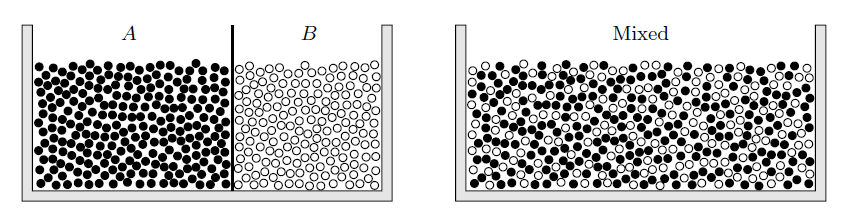
\includegraphics[width=0.75\linewidth]{images/fig4_1.png}
    \caption{두 종류의 분자가 섞이기 전후 모습이다.}
\end{figure}

첫 번째 근사로, 에너지나 부피의 변화는 무시하자. ($U$, $v$ fixed) 그러면 깁스 자유 에너지는 혼합 엔트로피에서 비롯할 것이다. 물질이 $x:1-x$로 존재하고 입자 총 개수는 $N$개임을 감안하자.
\begin{align}
    \Delta S_{\text{mixing}} &= k \ln [ {}_{N}C_{xN}] = k \ln \left[ \frac{N!}{(xN)! (N-xN)!} \right] \quad (\text{Strlling Approx.})\\
    &\approx k [ N \ln N - (xN) \ln(xN) - (N-xN) \ln (N-xN) ] \\
    &= -R[x\ln x + (1-x) \ln (1-x) ] \quad (\text{when }Nk \equiv R)
\end{align}
순수한 $A$와 $B$ 상태에서 1몰 당 깁스 자유에너지를 $G_A^\circ$, $G_B^\circ$라 하자. 깁스 자유 에너지에 대해선 다음이 성립한다.
\begin{align}
    G &= (1-x)G_A^\circ + xG_B^\circ  &(\text{No mixing})\\
    G &= (1-x)G_A^\circ + xG_B^\circ + \Delta S_{\text{mixing}} \cdot T &(\text{Ideal mixing})
\end{align}

\begin{figure}[h]
    \centering
    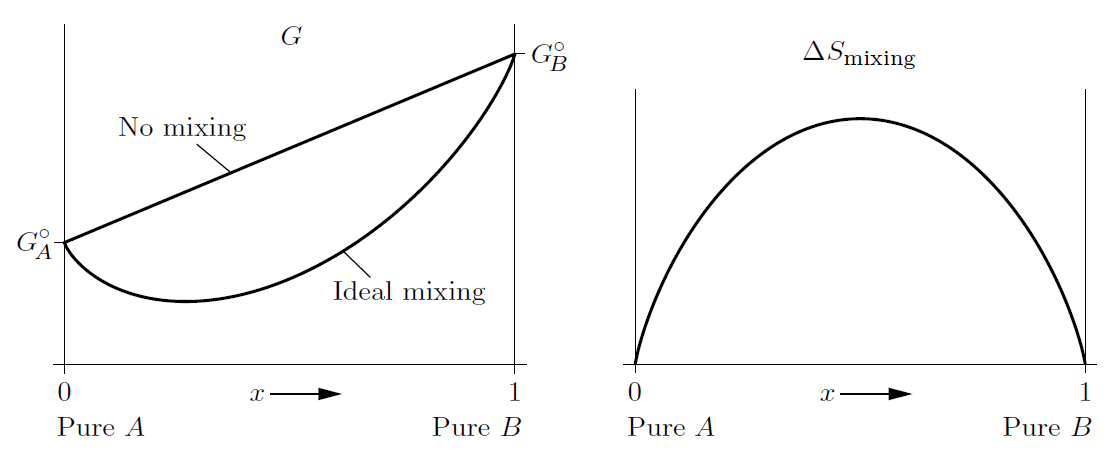
\includegraphics[width=0.7\linewidth]{images/fig4_2.png}
\end{figure}

유도한 바와 같이 simpie한 깁스 자유 에너지를 갖는 경우, \underline{ideal mixture}라고 한다. 실제로, $\Delta S_{\text{mixing}}$을 해석적으로 관찰할 경우, 다음과 같다.
\begin{equation}
    \frac{d}{dx} \Delta S_{\text{mixing}} \rightarrow \pm \infty \quad (\text{for }x \rightarrow 0, \ x \rightarrow 1)
\end{equation}
실제로, 구간의 endpoint들에선 기울기가 무한대로 발산해버리고, 이를 통해 \textcolor{blue}{equilibrium phase는 거의 항상 impurities를 갖고 있음}을 알수 있다. 만약, ideal하지 않게 섞이면 어떨까?

\newpage

\noindent
\textbf{Non-ideal Mixture}

만약, 혼합 과정에서 부피 변화를 무시할 때, $\Delta U_{\text{mixing}} \neq 0$이다!

\begin{figure}[h]
    \centering
    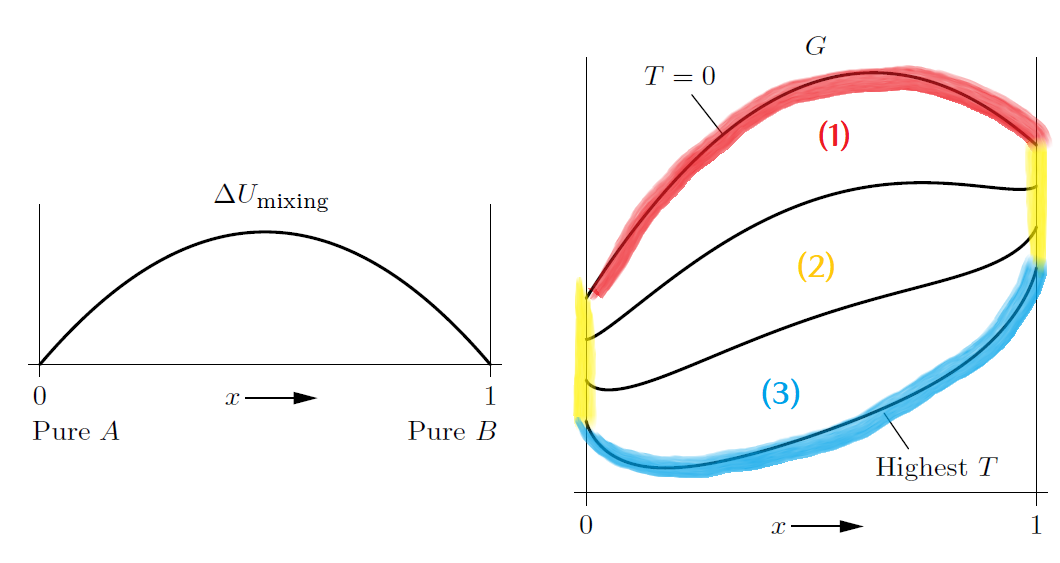
\includegraphics[width=0.7\linewidth]{images/fig4_3.png}
\end{figure}

\noindent
non-ideal한 상황에서, 깁스 자유 에너지는 다음과 같다.
\begin{equation}\label{eq:4-7}
    G = (1-x) G_A^\circ + xG_B^\circ + \color{blue} T \Delta S_{\text{mixing}} \color{black} + \color{red} \Delta U_{\text{mixing}} \color{black}
\end{equation}
(\ref{eq:4-7})은 위 그림의 3가지 경우에서 양상을 결정하는 항이 달라진다.
\begin{enumerate}
    \item[(1)] 구간에선 저온이고($T=0$), 이 땐, $U_{\text{mixing}}$이 dominate한다.
    \item[(2)] 와 같은 endpoint 근방에선 $\Delta S_{\text{mixing}}$이 dominate한다.
    \item[(3)] 구간에선 고온이고, 이 때 역시 $\Delta S_{\text{mixing}}$이 dominate한다.
\end{enumerate}

\begin{figure}[h]
    \centering
    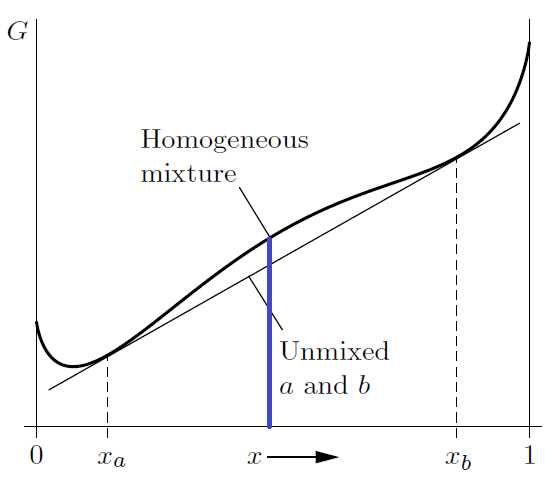
\includegraphics[width=0.4\linewidth]{images/fig4_4.png}
\end{figure}

위 깁스 자유에너지 그래프에서, 아래로 볼록한 두 구간의 양 끝에서 곡선에 접하는 가장 낮은 직선을 그려야 한다. 또한, 접선이 만나는 조성 구간 사이에서는, 혼합물이 자발적으로 $x_a$, $x_b$ 조성을 가진 두 상으로 분리된다. 그리고 특정 조성 $x$에 대해, 곡선에 접하는 직선이 가장 낮은 깁스 자유에너지 값을 준다.

우리는, $x_a$과 $x_b$ 사이 간격을 solubility gap이라 한다. 또한, 그 gap 안에 있는 상태를 immiscible하다 하고, 아닌 경우를 miscible하다고 한다. 아래 그림에서 왼쪽은 miscible, 오른쪽은 immiscible하다.

\begin{figure}[h]
    \centering
    
\includegraphics[width=0.75\linewidth]{images/fig4_5.png}
\end{figure}

\newpage

고체에서는, 두 물질을 혼합하면 보통 결정 격자에 큰 변형을 주어 에너지가 크게 증가하게 된다.

\begin{figure}[h]
    \centering
    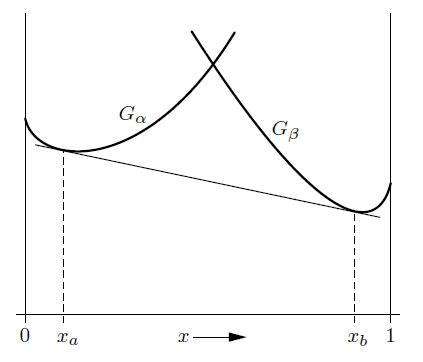
\includegraphics[width=0.4\linewidth]{images/fig4_7.png}
\end{figure}

\noindent
\textbf{Phase changes of a miscible mixture}

액체 질소와 액체 산소는 완전히 서로 섞일 수 있으므로, 액체 혼합물의 자유에너지 함수는 전체적으로 오목하다. 기체 혼합물의 자유에너지 역시 전체적으로 오목하다. 이 두 자유에너지 함수의 관계를 다양한 온도에서 비교해 보면, 시스템의 움직임과 phase diagram을 그릴 수 있다.

\begin{figure}[h]
    \centering
    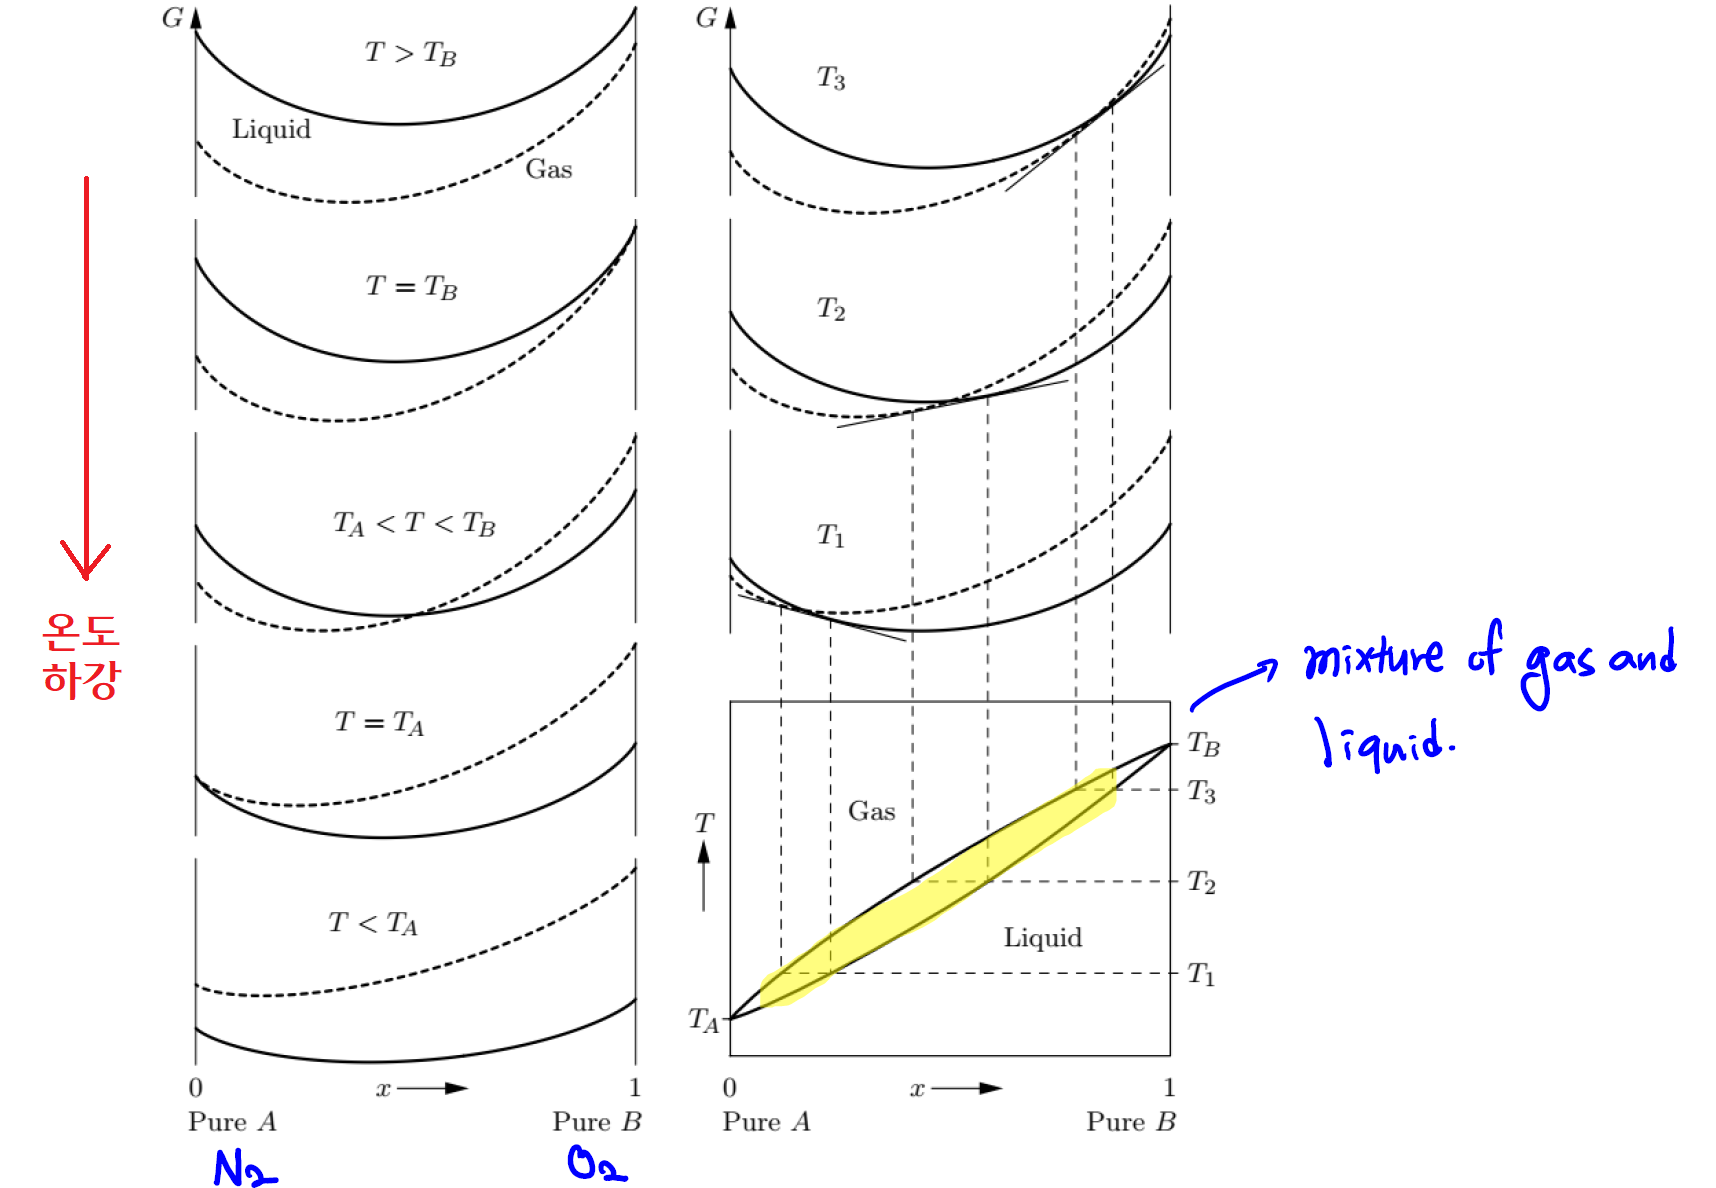
\includegraphics[width=0.9\linewidth]{images/fig4_8.png}
\end{figure}

엔트로피 $S>0$이고, 온도 $T$가 감소할 때, 다음의 identity를 떠올리자.
\begin{equation}
    \frac{\partial G}{\partial T} = -S
\end{equation}
이 경우, 깁스 자유 에너지는 증가한다. 또한, $S_{\text{gas}} > S_{\text{liquid}}$로부터, gas의 깁스 자유 에너지는 아주 빠르게 증가함.

\newpage

\begin{figure}[h]
    \centering
    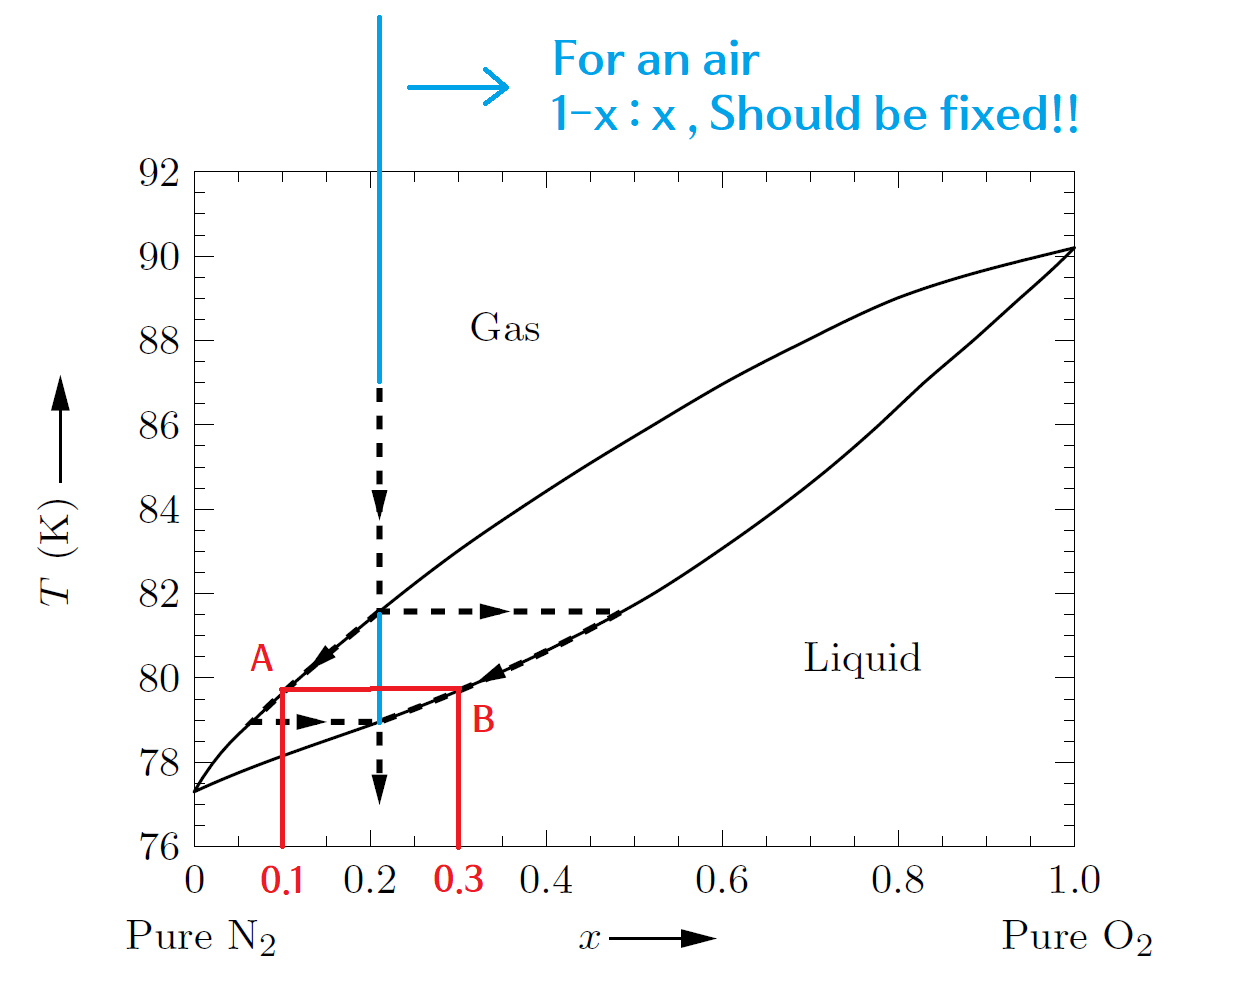
\includegraphics[width=0.67\linewidth]{images/fig4_9.png}
\end{figure}
\noindent
하늘색 점선의 경우, 대기의 조성비에 가깝도록 $x=0.21$정도로 설정한 선이다. 예를 들어, $T = 80$K에서, 는 기체와 액체 상태가 공존하는데, 기체의 경우 점 A처럼 산소 10\% + 질소 90\%로 존재하고, 액체는 점 B처럼 산소 30\%, 질소 70\%로 
혼합되어 존재한다. 또한, 양의 비율은 $A : B$로 주어진다.

\vspace{3mm}\noindent
\textbf{Phase changes of a eutectic system}

A와 B가 액체 상태에서는 완전히 섞일 수 있지만, 고체 상태에서는 서로 섞이지 않는 시스템의 고체–액체 상전이를 생각해보자. 이런 계의 이름을 공정계(eutectic system)라고 한다.

\begin{figure}[h]
    \centering
    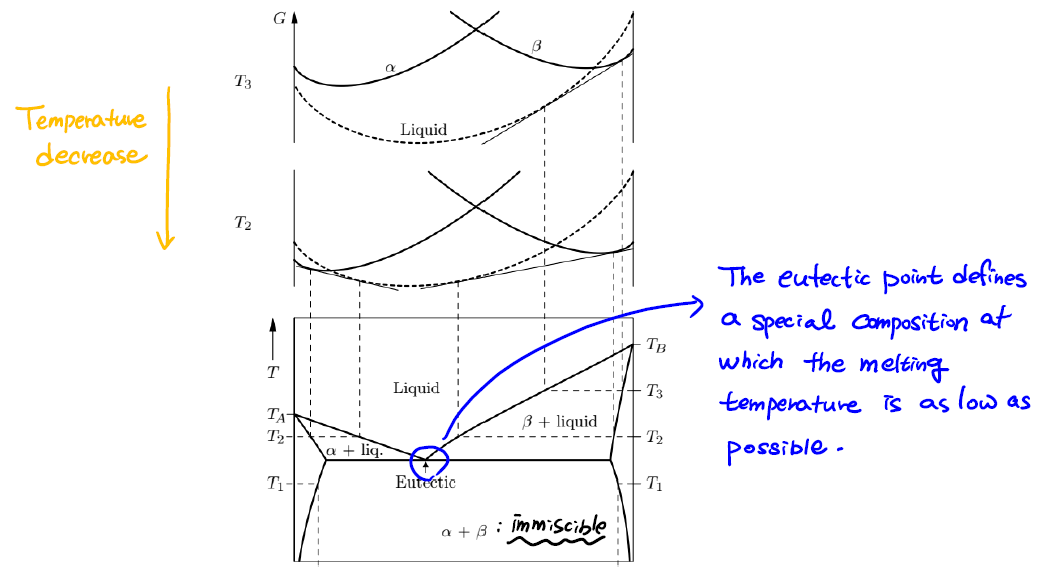
\includegraphics[width=1\linewidth]{images/fig4_10.png}
\end{figure}

공정점(eutectic point)은 녹는 온도가 가장 낮아지는 특별한 조성을 의미한다.

\newpage

\section{Dilute Solutions}

희석된 용액은 혼합물과 비슷하면서도, 용매를 주성분으로 본다는 점에서 차이가 있다. 용질 분자의 수가 용매 분자에 비해 훨씬 적을 때 용액이 희석(dilute)되었다고 한다. 

\begin{figure}[h]
    \centering
    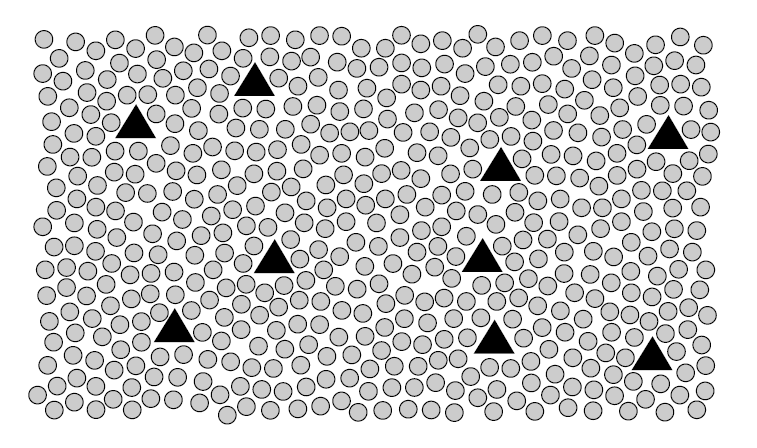
\includegraphics[width=0.4\linewidth]{images/fig5_1.png}
\end{figure}


순수한 용매에 대한 A 분자의 깁스 자유 에너지는 다음과 같다.
\begin{equation}
    G = N_A \mu_0 (T,P) \quad (\mu_0 \text{ is chem. potential in pure solvent})
\end{equation}
이제, 여기에 $B$ 분자를 더한다 가정하자. ($N_B \ll N_A$) 이 때, 온도와 압력은 고정한다.
\begin{equation}
    dG = dU + PdV - TdS = N_B = f(T,P) -TdS
\end{equation}
고정 조건들에 의해 $f(T,P)$가 생긴다. Mixing에 대한 엔트로피도 해석해보자.
\begin{align}
    dS = dS_{\text{mixing}} &= k \ln \binom{N_A + N_B}{N_B} = k \ln \frac{(N_A + N_B)!}{N_A ! N_B !}\\
    &\approx k [ (N_A + N_B) \ln (N_A + N_B) - N_A \ln N_A - N_B \ln N_B]\\
    &= k \left[ N_A \ln \left( \frac{N_A + N_B}{N_A} \right) + N_B \ln \left( \frac{N_A + N_B}{N_B} \right) \right]\\
    &\approx k \left[ N_A \cdot \frac{N_B}{N_A} + N_B \ln N_A - N_B \ln N_B \right]\\
    &= k [N_B + N_B \ln N_A - N_B \ln N_B]
\end{align}
따라서, mixing 깁스 자유에너지는 다음과 같다.
\begin{align}
    G_{\text{mixing}} &= N_A \mu_0 (T,P) + dG_{\text{mixing}}\\
    &= N_A \mu_0 (T,P) + N_B f(T,P) - N_B kT \ln N_A + N_B kT \ln N_B - N_B kT
\end{align}
따라서, 우리는 용매와 용질의 화학 퍼텐셜을 계산할 수 있다. $\mu_A$는 용매, $\mu_B$는 용질에 대한 값이다.
\begin{align} \label{eq:5-10}
    \mu_A &= \left( \frac{\partial G}{\partial N_A} \right)_{T,P,N_B} = \mu_0 (T,P) - \frac{N_B kT}{N_A}\\
    \mu_B &= \left( \frac{\partial G}{\partial N_B} \right)_{T,P,N_A} = f(T,P) + kT \ln (N_B / N_A)
\end{align}
용매의 화학 퍼텐셜에서, 용질이 많아질 수록 $\mu_A$는 감소한다. 또한, 용질의 화학 퍼텐셜은 다음 이상기체의 화학 퍼텐셜 공식과 유사하다.
\begin{equation}
    \mu_(T,P) = \mu^\circ (T) + kT \ln (P/P^\circ)
\end{equation}
다음으로 넘어가기 전, 농도에 대해 얘기하자면, 몰농도(molarity)는 \underline{용액 1L 당 용질의 몰수}, 몰랄농도(molality)는 \underline{용매 1kg 당 용질의 몰수}이다.

\newpage

따라서, 용액의 몰랄농도를 $m$이라 하자.\footnote{일반적으로 몰 농도는 $M$, 몰랄 농도는 $m$을 자주 사용한다.} 그러면 $\mu_B$는 다음과 같다.
\begin{equation}
    \mu_B = \left( \frac{\partial G}{\partial N_B} \right)_{T,P,N_A} = f(T,P) + kT \ln (N_B / N_A) = \mu_B^\circ (T,P) + kT \ln m_B
\end{equation}
여기서, $\mu_B^\circ (T,P)$는 용질 B의 몰랄 농도 $m=1$일 때의 화학 퍼텐셜이다.\footnote{표준 상태라고도 부른다.}

\vspace{3mm}\noindent
\textbf{Application of $\mu_A, \mu_B$ in solutions (Osmotic pressure)}

\begin{figure}[h]
    \centering
    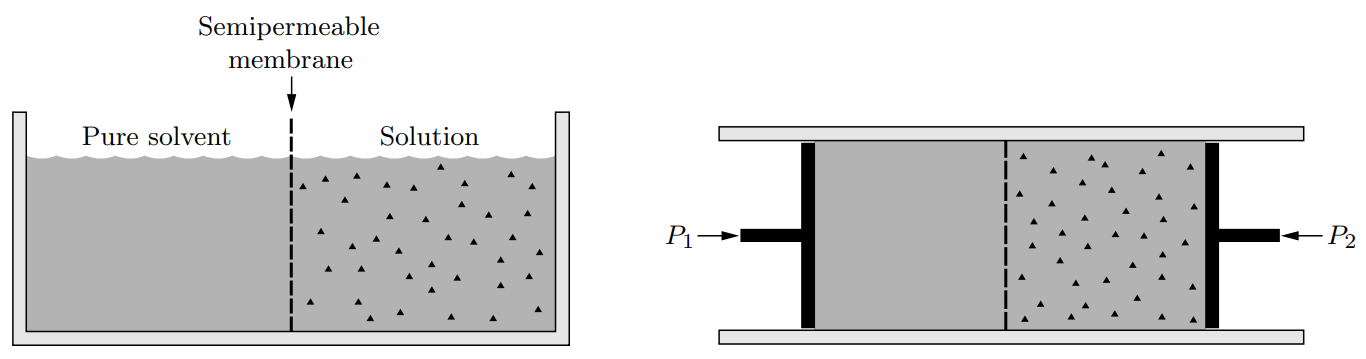
\includegraphics[width=0.9\linewidth]{images/fig5_2.png}
\end{figure}

우리가 먼 옛날 생물 시간에 배웠던 삼투압(Osmotic pressure)에 대해 알아보도록 하자. 왼쪽 그림은 용매 분자만 통과 가능한 반투과성 막으로 갈라져있다. 용액 내 용매의 화학 퍼텐셜은 순수 용매보다 낮다. 입자들은 화학 퍼텐셜이 더 낮은 쪽으로 흐르기에, 용매 분자들이 순수 용매 쪽에서 용액 쪽으로 자발적으로 이동한다.

우리는 오른쪽 그림처럼 적당한 압력을 가해 삼투압을 막아보고자 한다. (\ref{eq:5-10})을 통해 화학 퍼텐셜 차와 압력을 통해 식을 세우면 다음과 같다.
\begin{equation}
    \mu_0 (T,P_1) = \mu_0 (T,P_2) - \frac{N_B kT}{N_A}
\end{equation}
여기서, 두 압력이 그리 크지 않다고 가정하자. 근사를 때릴 수 있다.
\begin{equation}
    \mu_0 (T, P_2) \approx \mu_0 (T, P_1) + (P_2 - P_1) \frac{\partial \mu_0}{\partial P}
    \quad \Rightarrow \quad (P_2 - P_1) \frac{\partial \mu_0}{\partial P} = \frac{N_B kT}{N_A}
\end{equation}
고정된 $T,N$에 대해 다음 관계식이 성립한다.
\begin{equation}
    \frac{\partial \mu_0}{\partial P} = \frac{\partial }{\partial P} \frac{G_0}{N_A} = \frac{1}{N_A} \frac{\partial G_0}{\partial P} = \frac{V}{N_A}
\end{equation}
두 식을 연립해주면 다음을 얻는다.
\begin{equation}\label{eq:5-17}
    \boxed{P_2 - P_1 = \frac{N_B kT}{V} = \frac{n_B RT}{V}} \quad (\text{$P_2-P_1$은 삼투압})
\end{equation}
(\ref{eq:5-17})의 관계를 \textcolor{blue}{반트호프 공식(Van't Hoff's formula)}라고 한다.

\newpage

\noindent
\textbf{Application of $\mu_A, \mu_B$ in solutions \textcolor{blue}{(Boling and freezing points)}}

\begin{figure}[h]
    \centering
    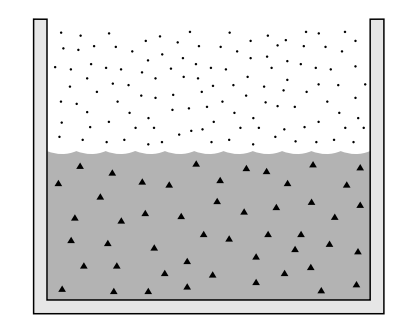
\includegraphics[width=0.3\linewidth]{images/fig5_3.png}
\end{figure}

용질이 존재하면 용매가 증발하려는 경향이 줄어든다. 그림은 용매 분자 A와 용질 분자 B가 존재하는 양상을 나타낸다. 고등학교 화학2에서 배웠던 증기압에 의한 용액의 총괄성 얘기다.

화학 퍼텐셜에 대한 평형 조건(equilibrium condition)은 다음과 같다. 
\begin{equation}
    \mu_{A,\mathrm{liq}}(T, P) = \mu_{A,\mathrm{gas}}(T, P) \quad \Rightarrow \quad \mu_0(T, P) - \frac{N_B k T}{N_A} = \mu_{\mathrm{gas}}(T, P)
\end{equation}
$\mu$ 함수를 순수한 용매($P^\circ$) 근방에서 테일러 전개하여 라울 법칙을 유도해보자.
\begin{equation}
    \cancel{\mu_0 (T,P_0)} + (P - P_0) \frac{\partial \mu_0}{\partial P} - \frac{N_B kT}{N_A} = \cancel{\mu_\text{gas} (T,P_0)} + (P -P_0) \frac{\partial \mu_\text{gas}}{\partial P}
\end{equation}
$(\partial \mu / \partial P) = (V/N)$임을 이용하자.
\begin{equation}
    (P - P_0) \left( \frac{V}{N} \right)_{\text{liq}} - \frac{N_B kT }{N_A} = (P - P_0) \left( \frac{V}{N} \right)_{\text{gas}}
\end{equation}
$(V/N)$의 값은 gas일 때가 liq일 때보다 압도적으로 크고, gas에선 $kT/P_0$이므로,
\begin{equation}
    P - P_0 = -\frac{N_B}{N_A} P_0 \quad \Rightarrow \quad \boxed{\frac{P}{P_0} = 1-\frac{N_B}{N_A}} \quad \text{(Raoult's law)}
\end{equation}
분자들의 모형으로 해석하면, 증기압이 감소하는 이유는 용질을 첨가하면 액체 표면에 있는 용매 분자의 수가 줄어들기 때문이다.

우리는 등압 상태로 가정하여 화학 퍼텐셜 평형 조건을 통해 끓는점 오름도 살펴볼 수 있다. 끓는점이 $T_0$면,
\begin{equation}
    \mu_0 (T_0, P) + (T-T_0) \frac{\partial \mu_0}{\partial T} - \frac{N_B kT}{N_A} = \mu_\text{gas} (T_0, P) + (T-T_0) \frac{\partial \mu_\text{gas}}{\partial T}
\end{equation}
$(\partial G / \partial T) = -S$임을 이용하자.
\begin{equation}
    -(T-T_0) \left( \frac{S}{N} \right)_{\text{liq}} - \frac{N_B kT}{N_A} = - (T- T_0) \left( \frac{S}{N} \right)_{\text{gas}}
\end{equation}
$S_\text{gas} - S_\text{liq} = L/T_0$이다. 따라서, $T\approx T_0$도 이용하면, 다음과 같이 끓는점 오름을 설명할 수 있다.
\begin{equation}
    T - T_0 = \frac{N_B kT \cdot T_0}{L} \approx \frac{N_B kT_0^2}{L} = \frac{n_B R T_0^2}{L}
\end{equation}


\newpage

\section{Chemical Equilibrium}

먼저, 가역 반응인 물의 자동 이온화를 생각해보자.
\begin{equation}
    \ch{H2 O} \leftrightarrow \ch{H+} + \ch{OH-}
\end{equation}
깁스 자유에너지의 측면에서, 이온들의 존재에 의해 엔트로피가 증가하기 떄문에 깁스 자유에너지가 줄어들 것이다.

\begin{figure}[h]
    \centering
    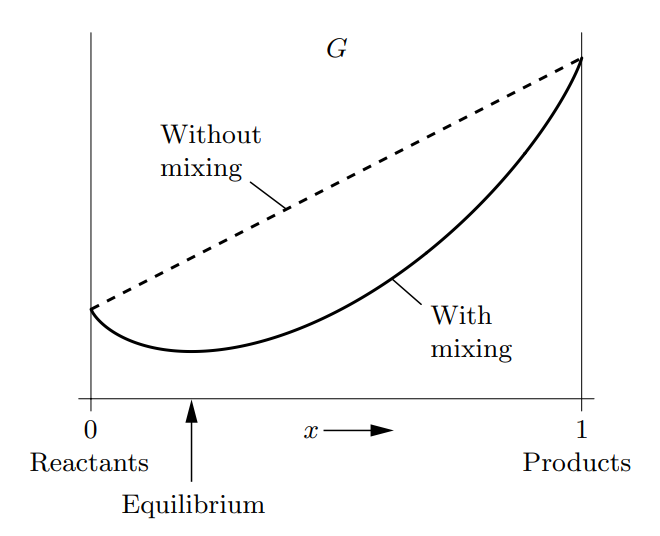
\includegraphics[width=0.45\linewidth]{images/fig6_1.png}
\end{figure}

평형 상태에서 다음 조건을 만족한다.
\begin{equation}\label{eq:6-2}
    0 = dG = \sum_i \mu_i dN_i = \mu_{\ch{H2O}} N_{\ch{H2O}} + \mu_{\ch{H+}} N_{\ch{H+}} + \mu_{\ch{OH-}} N_{\ch{OH-}}
\end{equation}
여기서, 화학 반응식에 의해 $dN$은 순서대로 각각 -1, +1, +1로 결정된다. 이를 (\ref{eq:6-2})에 대입하면 평형 조건은
\begin{equation}
    \mu_{\ch{H2O}} = \mu_{\ch{H+}} + \mu_{\ch{OH-}}
\end{equation}
이다. 이제, 일반적인 반응의 평형 조건으로 확장해보자. 
\begin{equation}
        \nu_1 X_1 + \nu_2 X_2 + \cdots \leftrightarrow \nu_3 X_3 + \nu_4 X_4 + \cdots
\end{equation}
라는 반응식에서, 다음과 같이 평형 조건이 건설된다.
\begin{equation}
    \nu_1 \mu_1 + \nu_2 \mu_2 + \cdots = \nu_3 \mu_3 + \nu_4 \mu_4 + \cdots
\end{equation}
화학 퍼텐셜에 대한 식을 다시 정리해보자.
\begin{itemize}
    \item \textbf{Gas} : $\mu_\text{gas} = \mu^\circ + kT \ln (P/P^\circ)$
    \item \textbf{Solvent} : $\mu_A = \mu_0 (T,P) - \dfrac{N_B kT}{N_A}$
    \item \textbf{Solute} : $\mu_B = \mu^\circ (T,P) + kT \ln (m_B)$
\end{itemize}
우리는 4가지 예시를 들 수 있는데, 질소 고정, 물의 해리, 산소의 물 속 용해, 수소의 이온화이다. 하나씩 알아보면서 5장을 마무리짓도록 하자.

\newpage

\noindent
\textbf{1. Nitrogen fixation (gas)}

\begin{figure}[h]
    \centering
    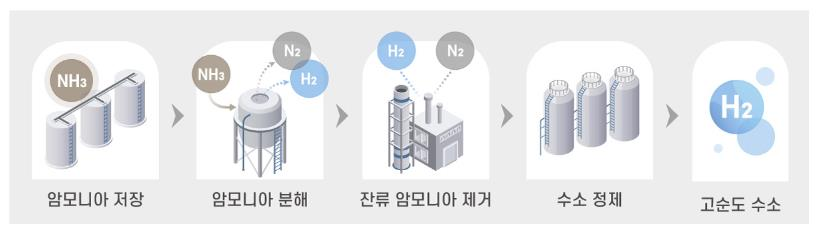
\includegraphics[width=0.65\linewidth]{images/fig6_2.png}
\end{figure}

화학 반응식과 그에 따른 평형 조건은 다음과 같다.
\begin{equation}
    \ch{N2} + \ch{3 H2} \leftrightarrow \ch{2 NH3} \quad / \quad \mu_{\ch{N2}} + 3\mu_{\ch{H2}} = 2\mu_{\ch{NH3}}
\end{equation}
이상기체에서, $\mu_\text{gas} = \mu^\circ + kT \ln (P/P^\circ)$이므로, 이를 이용하면
\begin{align}
    \mu_{\ch{N2}}^\circ + kT \ln \left( \frac{P_{\ch{N2}}}{P^\circ} \right) + 3\mu_{\ch{H2}} + 3kT \ln \left( \frac{P_{\ch{H2}}}{P^\circ} \right) &= 2\mu_{\ch{NH3}} + 2 kT \left( \frac{P_{\ch{NH3}}}{P^\circ} \right)\\
    kT \ln \left( \frac{P_{\ch{N2}}}{P^\circ} \right) + 3kT \ln \left( \frac{P_{\ch{H2}}}{P^\circ} \right) -2 kT \left( \frac{P_{\ch{NH3}}}{P^\circ} \right) &= 2\mu_{\ch{NH3}} -\mu_{\ch{N2}}^\circ -3\mu_{\ch{H2}}
\end{align}
양 변에 아보가드로 수를 곱해서 정리하면 다음과 같다.
\begin{equation}
    RT \ln \left( \frac{P_{\ch{N2}} P_{\ch{H2}}^3}{P_{\ch{NH3}}^2 (P^\circ)^2} \right) = \Delta G^\circ \quad \Rightarrow \quad \boxed{\frac{P_{\ch{N2}} P_{\ch{H2}}^3}{P_{\ch{NH3}}^2 (P^\circ)^2} = e^{-\Delta G^\circ /RT} \equiv K(T)}
\end{equation}
$K(T)$를 우리는 \underline{평형 상수}라고 한다. 평형 상수는 고온에서 작아진다. 그러면 저온에서 암모니아를 다루는게 이득 아니냐? 생각하겠지만, 평형 조건은 반응 속도에 무관하기 때문에 상관 없다.

\vspace{3mm}\noindent
\textbf{2. Dissociation of Water (solution)}

앞서 봤던 물의 분해 반응식과 평형 조건을 가져오자.
\begin{equation}
    \ch{H2 O} \leftrightarrow \ch{H+} + \ch{OH-} \quad / \quad \mu_{\ch{H2O}} = \mu_{\ch{H+}} + \mu_{\ch{OH-}}
\end{equation}
분해가 묽은 용액에서 일어난다는 조건은 수식적으로 아주 좋은 근사 조건이다. 앞서 봤던 용액의 화학 퍼텐셜 조건을 이용하면 다음이 성립한다.
\begin{align}
    \text{Solvent} &: \mu_A = \mu_0 (T,P) - \frac{N_B kT}{N_A}\\
    \text{Solute} &: \mu^\circ (T,P) + kT \ln m_B
\end{align}
이를 통해 다음과 같은 평형 조건을 얻을 수 있다.
\begin{equation}
    \mu_{\ch{H2 O}}^\circ = \mu_{\ch{H+}}^\circ + kT \ln m_{\ch{H+}} + \mu_{\ch{OH-}}^\circ + kT\ln m_{\ch{OH-}}
\end{equation}
양 변에 아보가드로 수 $N_A$를 곱하여 정리하면 다음과 같다.
\begin{equation}
    RT \ln (m_{\ch{H+}} \cdot m_{\ch{OH-}}) = -N_A (\mu_{\ch{H+}}^\circ + \mu_{\ch{OH-}}^\circ - \mu_{\ch{H2 O}}^\circ) = -\Delta G^\circ  \quad \Rightarrow \quad m_{\ch{H+}} \cdot m_{\ch{OH-}} = e^{-\Delta G^\circ / RT}
\end{equation}
Circ의 조건은 물은 순수한 물, 이온들은 1m의 몰랄농도일 때이다. 여기서, 고등학교 화학 1에서 배웠던 수소이온농도지수(pH)를 정의할 수 있는데,  알아둬야 하는 것은, \underline{엄밀히 pH는 몰랄 농도로 정의해야 한다}는 것이다!!\footnote{고교 화학에선 수소 이온의 몰 농도로 정의한다.}
\begin{equation}
    \boxed{\text{pH} \equiv -\log_{10} m_{\ch{H+}}}
\end{equation}

\newpage

\noindent
\textbf{3. Oxygen dissolving in water (gas, solution)}

\begin{figure}[h]
    \centering
    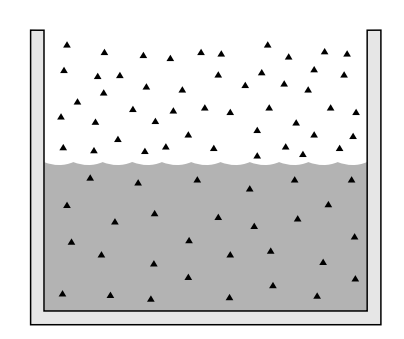
\includegraphics[width=0.3\linewidth]{images/fig6_3.png}
\end{figure}

그림에서 일어나는 반응과, 표준 깁스 자유 에너지는 다음과 같다.
\begin{equation}
    \ch{O2} (g) \leftrightarrow \ch{O2} (aq), \quad \Delta G^\circ = 164\text{kJ}
\end{equation}
따라서, 평형 조건에선 $\mu_\text{gas} = \mu_\text{solute}$여야 하므로 다음이 성립한다.
\begin{equation}
    \mu_\text{gas}^\circ  + kT \ln \left( \frac{P}{P^\circ} \right) = \mu_\text{solute}^\circ + kT \ln m
\end{equation}
양 변에 아보가드로 수 $N_A$를 곱하여 정리하면 다음과 같다.
\begin{align}
    RT \ln \left( \frac{P/P^\circ}{m} \right) = N_A (\mu_\text{solute}^\circ - \mu_\text{gas}^\circ) = \Delta G^\circ \quad \Rightarrow \boxed{\frac{m}{P/P^\circ} = e^{-\Delta G\circ / RT}}
\end{align}
몰랄 농도와 $P,T$의 관계를 헨리 법칙(Henly's law)라고 한다.

\vspace{3mm} \noindent
\textbf{4. Ionization of hydrogen (gas, plasma)}

수소의 이온화 반응식과 평형 조건은 다음과 같다. (p는 proton, e는 electron이다.)
\begin{equation}\label{eq:6-19}
    \ch{H} \leftrightarrow \ch{p} + \ch{e} \quad / \quad kT \ln \left( \frac{P_\text{H} P^\circ}{P_\text{p} P_\text{e}} \right) = \mu_\text{p}^\circ + \mu_\text{e}^\circ - \mu_\text{H}^\circ
\end{equation}
단원자 이상기체의 화학 퍼텐셜 값을 적용하면 다음과 같다.
\begin{equation}
    \mu = -kT \ln \left[ \frac{V}{N} \left( \frac{2 \pi m k T}{h^2} \right)^{3/2} \right]
= -kT \ln \left[ \frac{kT}{P} \left( \frac{2 \pi m k T}{h^2} \right)^{3/2} \right]
\end{equation}
수소의 이온화 에너지 $I= 13.6$eV를 취해보도록 하자. 이를 (\ref{eq:6-19})에 대입하자.
\begin{equation}
    kT \ln\left( \frac{P_H P^\circ}{P_P P_e} \right) = -kT \ln \left[ \frac{kT}{P^\circ} \left( \frac{2\pi m_\text{P} kT}{h^2} \right)^{3/2} \right]- \cancel{ kT \ln \left[ \frac{2\pi m_\text{e} kT}{h^2} \right]^{3/2}} + \cancel{kT \ln \left[ \frac{kT}{P^\circ} \left( \frac{2\pi m_\text{H} kT}{h^2} \right)^{3/2} \right]} + I
\end{equation}
따라서, 간단히 정리하면 다음과 같은 관계를 얻을 수 있다.
\begin{equation}
    - \ln \left( \frac{P_\text{H} P^\circ}{P_\text{P} P_e} \right) = \ln \left[ \frac{kT}{P^\circ} \left( \frac{2\pi m_e kT}{h^2} \right)^{3/2} \right] - \frac{I}{kT}
\end{equation}
최종적으로, 수소의 이온화 정도를 나타낸 비율은 다음과 같다.
\begin{equation}\label{eq:6-23}
    \boxed{\frac{P_\text{P}}{P_\text{H}} = \frac{kT}{P_e} \left( \frac{2\pi m_e kT}{h^2} \right)^{3/2} e^{-I/kT}}
\end{equation}
(\ref{eq:6-23})의 관계를 사하 방정식(Saha equation)이라 한다. 이는 고온 플라즈마에서 수소가 얼만큼 이온화되었는지 알려주는 지표로써 사용할 수 있다.



\end{document}